\section{Controlled numerical Simulations}
\textbf{Two different types of simulations are involved in this work, namely cosmological (see side projects in Appendix B) and controlled sims (described in this section). Both types are produced by using the GADGET-2 code (Springel 2005). The cosmological simulation is just analyzed, whereas the controlled simulations are both performed (inside a non-cosmological Newtonian box) and subsequently analyzed. By the name controlled it is meant that the sim. is more local and does not take an expanding spacetime into account. This enables a more detailed study where hierarchical clustering, mergers, build-up of halo sub-structure and accretion effects does not wash out the potential attractors of interest. The controlled sims is comprised of two types, namely I (An instantaneous change of the gravitational potential) and II (Energy exchange) which is further varied in four principal ways (cartesian, radial, tangential and total velocity perturbations).} \\ \\

\textit{When looking for universalities it is crucial to start from many different IC's. It is equally important to perturb these IC's in a variety of ways in order to make sure any found universalities is not an artifact of some artificial computer method. For this reason structures are subjected both to Sims. of type I and II. Both types have an underlying structure in common: Structures are perturbed and then gravity is allowed to work on them during subsequent simulation. This} perturbation$\rightarrow$simulation \textbf{method is kept under all numerical experiments in this work. They both serve to mimic the effects dominant during galaxy mergers since these dramatic events can alter characteristic features of the galaxies surrounding dark matter halos. It will then become more clear if these halos are driven towards any preferred state or configuration.} \\ \\

\centerline{\textbf{Particle number}} 
Particle number is steadily increased from $10^4$ to $10^5$ and finally all the way to $10^6$. To compute for example the velocity dispersion $\sigma$ or the density $\rho$ for a structure divided into 20 radial bins, and to get a good statistical result, $5\cdot 10^2$ particles is needed in each bin and therefore a minimum of $10^4$ particles must be included. However, in order to determine derived or constructed quantities such as $\kappa$ or $\gamma$, a minimum of $5\cdot 10^3$ particles in each of the 20 bins is more favorable and hence a total of $10^5$ particles is wanted. Looking at 2.nd order derivatives as for example in the project 'Bumpy road to universalities', even more particles must be included. A minimum of $5\cdot 10^4$ particles in each of the 20 bins is more favorable and hence a total of $10^6$ particles is wanted. \\

\centerline{\textbf{Gravitational softening}} 
For most cosmological simulations the softening depends upon the particle number in the following way [10]:
\begin{equation}
\epsilon \geq (\frac{3}{800\pi N^2})^{\frac{1}{3}}d  
\end{equation}
where d is the mean particle distance. For $N=5$, $\epsilon \geq \frac{1}{30}d$. For the controlled sims. it is simply assumed that $\epsilon$ scales as $N^{\frac{1}{3}}$. In Sparre and Hansens paper (\url{http://arxiv.org/abs/1210.2392}) a slightly smaller softening of 0.0050 were used in both the G-perturbations and the energy exchange simulations, It is therefore interesting to see if the attractor also exists if the above softening-values are used. This is expected to be the case, as a slightly larger softening only affects the very inner part. As a rule of thumb the softening must become 10 times larger when the particle number increases a thousand times [11]. \\ \\

\centerline{\textbf{Range of Jeans parameters}} 
For an Edd structure, $\beta = 0$ initially, and for an OM structure, $\beta \in [0,1]$. So the range of $\beta$ is set to $[0,1]$. For the density profile $\rho_{HQ}$, $\gamma \in [-3,-1]$, and for the density profile $\rho_{0,5}$, $\gamma \in [-5,0]$. The $\gamma$-range thus depends on the density profile under consideration.

\subsubsection{I: G-perturbations}
\textbf{To mimic the proces of violent relaxation during galaxy and cluster mergers this type of sim. creates an instantaneous change in the gravitational potential. Such a change perturbs the acceleration of each particle. This section gives a technical description of exactly how each structure was perturbed wrt the gravitational potential during this type of sim. The section gives an overview of a specific pattern of G-perturbations and following simulation, which is repeated a certain number of times, as well as an overview of the simulation times used during each step.} \\ \\

The purpose of the simulations of type I is to resemble the proces of violent relaxation during mergers. But instead of using the relation describing violent relaxation $\big(\frac{dE}{dt} = \frac{d\Phi}{dt}\big)$, where a time-dependence of the gravitational potential ($\Phi$) exists, a time variation of Newtons gravitational constant is applied, G(t). This effectively produces the same effect. After each perturbation of G from its standard value, the structures are simulated. This pattern continues for a certain amount of time until a new stable configuration is found. Practically, changes are made to the value of Newtons gravitational constant G from its standard value of $G = 6.67 \cdot 10^{-11} \frac{Nm^2}{kg^2}$ here corresponding to $G=1$ in non-SI units, to either 1.2 or 0.8 times the standard value, corresponding to an increase or decrease by 20 \%, or 1.05 to 0.95 times the standard value, corresponding to an increase or decrease by 5 \%. Either 20 or 5 pct is added or subtracted systematically from G in a certain pattern (see table 3). The Simulations always start out with $G = 1$ in Run 0 which last for 100 simulation times. This is done to give the structure time to work under its own gravity and make sure the IC's are set up correctly. It provides a way to see that the IC is in a stable configuration. The pattern from Run 1 to Run 5 is then repeated a certain number of times (see table 4). Ending up with runs of $G=1$ for longer time gives the structures better chance to reach stable equilibria (see tables 5-7). The idea behind changing the G-value by a smaller amount (5 pct.) from the standard value (as is the case with sim B) is to have the structure depart less from equilibrium during the simulations. It is seen later on in the analysis of the velocity distribution functions that these are not so different if the perturbations are larger or smaller, but the $\gamma$ vs. $\beta$ and $\gamma + \kappa$ vs. $\beta$ plots look slightly different if G is perturbed by 20\% or by 5\%. GADGET-2 makes a certain number of runs with varying values assigned to the gravitational constant G (Corresponding to perturbing the gravitational potential, i.e. An instantaneous change in $\Phi$ ). Most of these runs each produce 6 snapshot files, except for the last run in each simulation, where the time is increased from Timemax = 100 to Timemax = 2300 (giving 93 snapshots). The method of varying the potential corresponds to changing the accelerations of the individual particles. It is then interesting to see how the structures will respond, more on this in the next section: 'The attractor'. When the gravitational constant is lowered to the value of $ G = 0.8 $ and a structure is simulated by Gadget-2 for 100 time units, an expansion of that structure naturally occurs. When the gravitational constant is raised to the value of $ G = 1.2 $ and the structure again is simulated for 100 time units, A contraction of this structure now happens. This type of simulation where the structure pulsates is reminiscent of violent relaxation. \\ \\

\begin{table}[!htbp]
\centering
\begin{tabular}{|c|c|c|c|c|}
\hline
 Simulation    & A, $C_4$-$C_6$, $CS_4$-$CS_6$, $D_1$, $D_2$ and $DS_1$ & B          \\ \hline
 Run No.       &   G-value                                              &   G-value  \\ \hline
 0			   &     1.0                 						       &     1.0    \\ \hline
 1			   &     1.2    											   &     1.05   \\ \hline
 2			   &     0.8     										   &     0.95   \\ \hline
 3			   &     1.0   											   &     1.0    \\ \hline
 4			   & 	 1.0     										   &     1.0    \\ \hline
 5			   & 	 1.0     									       &     1.0    \\ \hline
\end{tabular}
\caption {Simulation I pattern. First this table states the name of each structure. The B structure is placed alone as it has a unique percentage of change to G of only $5 \%$, whereas the others all have G-perturbations to the order of $20 \%$. For each run a simulation time of 100 is used (corresponding to one dynamical time at $r=12.7r_s$). Left column numerates the different simulation runs. For all structures undergoing this type of simulation they are initially set up in the GADGET-2 code to be subjected to gravity with a potential corresponding to the standard value of G (here it means G=1). After the zeroth run  the simulation is paused and an increase of the G value (corresponding to a stronger gravitational potential) is applied, after which the simulation is continued. After the next 100 simulation times the G value is decreased (corresponding to a weaker potential) and the simulation is allowed to continue yet again for the next 100 simulation times. Finally G remains at the standard value for $3\cdot 100$ simulation times. This whole pattern or 'chunk' from run 1 to run 5 is then repeated a different number of times which can be seen in the following table.
}
\end{table}

\begin{table}[!htbp]
\centering
\begin{tabular}{|c|c|c|c|c|}
\hline
 Simulation                   & A & B and E & $C_4$-$C_6$ and $CS_4$-$CS_6$ & $D_1$, $D_2$ and $DS_1$ \\ \hline
 No. repetitions of pattern   & 9 & 39& 9 & 9 \\ \hline
\end{tabular}
\caption {Pattern repetitions. The 'chunks' of G-perturbations and subsequent simulations are repeated for the above stated number of times for all the different structures in question.}
\end{table}

\begin{table}[!htbp]
\centering
\begin{tabular}{|c|c|c|}
\hline
            & Simulation A, $C_4$-$C_6$ and $CS_4$-$CS_6$ &             \\ \hline
 Run        &     G                                       &  TimeMax    \\ \hline
 46         &    1.2                                      &    100      \\ \hline
 47         &    0.8                                      &    100      \\ \hline
 48         &    1.0                                      &    2300     \\ \hline   
\end{tabular}
\caption {Final runs. After the series of pattern repetitions shown before, for the here mentioned structures three final \textit{perturbation} $\rightarrow$ \textit{simulation} experiments are run: G is increased by $20 \%$ and structures are subjected to their self-gravity for 100 sim. times, G is decreased by $20 \%$ and structures are run for 100 sim. times and finally G is kept at unity and structures are run for 2300 sim. times in order to give the outer part of the structures more time to reach stable equilibria.}
\end{table}

\begin{table}[!htbp]
\centering
\begin{tabular}{|c|c|c|}
\hline
            & Simulation B and E &             \\ \hline
 Run        &     G              &  TimeMax    \\ \hline
 196        &    1.05            &    100      \\ \hline
 197        &    0.95            &    100      \\ \hline
 198        &    1.0             &    2300     \\ \hline   
 199        &    1.0             &    2300     \\ \hline  
\end{tabular}
\caption {Final runs. After the series of pattern repetitions shown before, for the here mentioned structures three final \textit{perturbation} $\rightarrow$ \textit{simulation} experiments are run: G is increased by $5 \%$ and structures are subjected to their self-gravity for 100 sim. times, G is decreased by $5 \%$ and structures are run for 100 sim. times and finally G is kept at unity and structures are run for $2\cdot 2300$ sim. times}
\end{table}

\begin{table}[!htbp]
\centering
\begin{tabular}{|c|c|c|}
\hline
            & Simulation $D_1$, $D_2$ and $DS_1$ &             \\ \hline
 Run        &     G                              &  TimeMax    \\ \hline
 49         &    1.0                             &    2300     \\ \hline   
\end{tabular}
\caption {Final run. After the series of pattern repetitions shown before, for the here mentioned structures one final \textit{perturbation} $\rightarrow$ \textit{simulation} experiments is run: G is kept at unity and the structures are run for 2300 sim. times}
\end{table}

\centerline{\textbf{Particle tracking}}
In order to test whether or not structures subjected to Sim. I has the tendency to expand systematically in the central region and throw out particles when pulsating as the effect of changing the gravitational potential, a few test particles has been chosen and tracked through a few different time-slices/snapshot-files of the simulations (See figure 10). In conclusion, there is no major systematic tendency of outward drift but only a small effect of turning initial cuspy profiles into profiles with small cores.

\begin{figure}[!htbp]
\centering
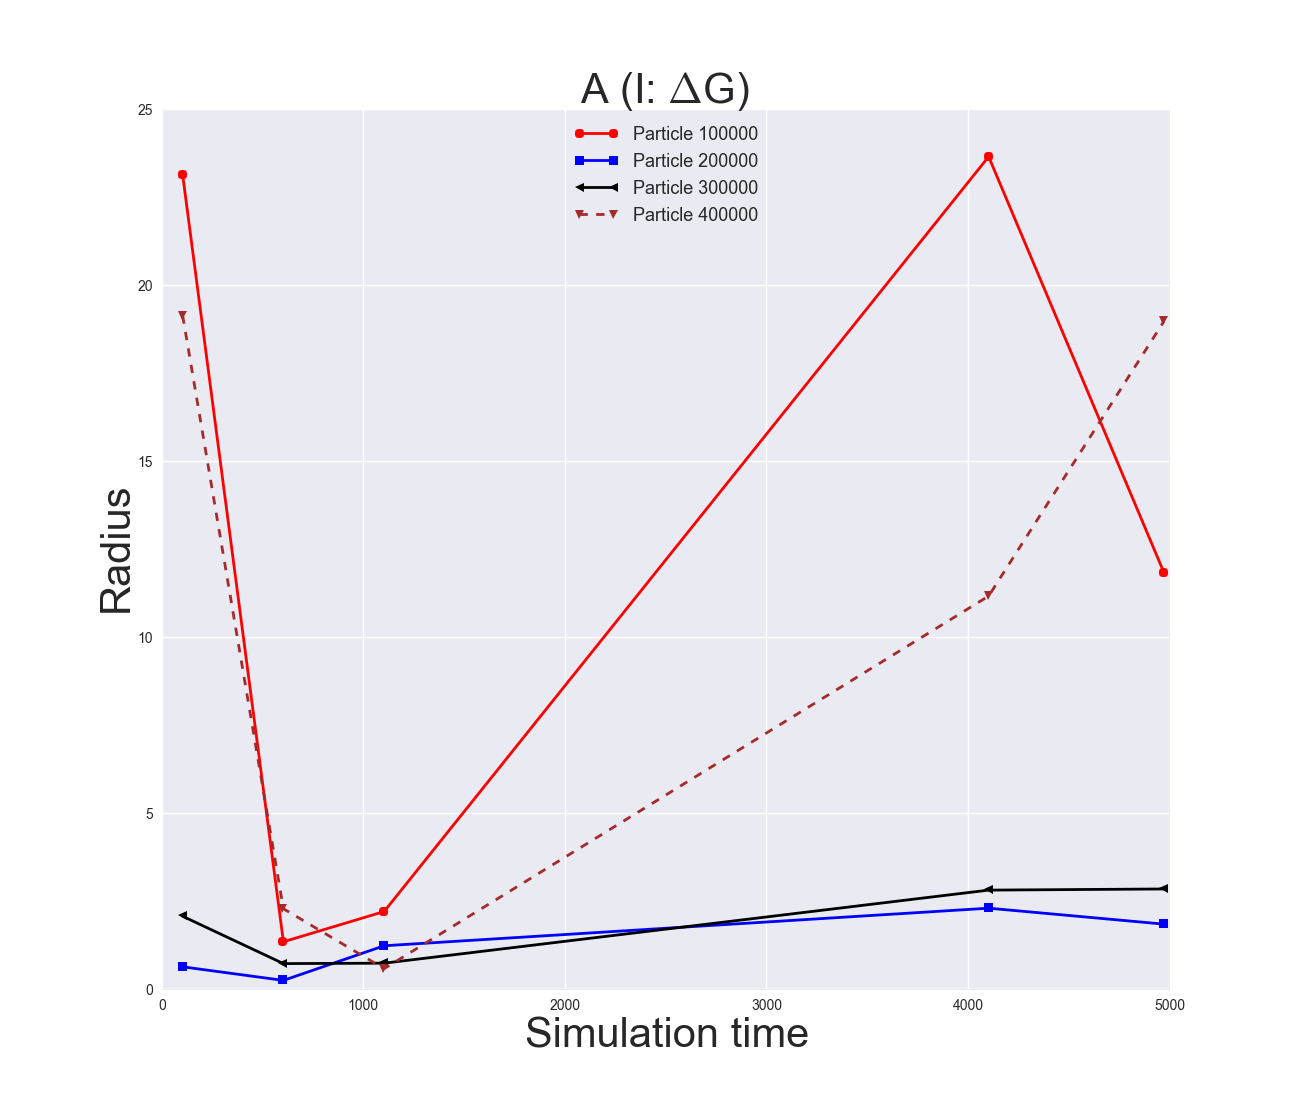
\includegraphics[width=1.0\linewidth]{img/Fig_combine_ASCII_A.png}
\caption{Time evolution of radius for a few chosen particles (ID's $10^5$, $2\cdot10^5$, $3\cdot10^5$ and $4\cdot10^5$) is plotted for selected snapshot files (IC, 5$\_$005, 10$\_$005, 40$\_$005 and 48$\_$009) of Sim. I for structure A. The figure shows that there is no systematic tendency of neither outward nor inward drift as indicated by all four particles changing radius in a stochastic manner as time evolves. This is expected due to the pulsating effect the G-perturbations has on structures.}
\label{fig:test}
\end{figure}

\centerline{\textbf{Total velocity profile}} 
As all structures have a scale-radius of unity, $r_s = 1$, the total velocity distribution is centered around unity as well (See figure 11). Over time however, substructure is created as we notice the emergence of filaments or 'fingers', each finger corresponding to an increase in the gravitational potential thus increasing individual particle accelerations and their contribution to the overall total velocity distribution is to drift outwards towards larger radii in this characteristic filament pattern. (see figure 12 and 13). 

\centerline{\textbf{Final density}} 
Figure 14 shows the flattening of structures as their density profiles go from cuspy to cored over the duration of the simulations. Final structures in average have cores with a size of $\log \frac{r}{r_{-2}} = -0.5$, i.e. $\frac{r}{r_{-2}} \approx 0.32$ or put in other words the cores span 32 \% of $r_{-2}$, the radius where $\gamma = -2$ (for a HQ profile this equals the scale radius, $r_{-2} = r_s$). \\
\centerline{\textbf{Structures become anisotropic over time}} \\
In figure 15 the effect this sim. type I has on velocity anisotropy can be seen. All structures will over time grow radially biased wrt. the $\beta$-profile no matter if they belong to Edd or OM ICs. \\
\centerline{\textbf{Density slope extremas}} \\
Figure 16 reveals an interesting feature of final $\gamma$ shapes. notice in the outer part how there seem to be distinct bumps and wiggles. This is explored further in the side project found in App. B.4 'The bumpy road to universalities' where different normalizations are carried out to look for universalities in the final $\gamma$-profiles which seem to poses up to 6 unique local extremas (3 minima and 3 maxima). \\
\centerline{\textit{Evolution of radial velocity dispersion}} \\
Figure 17 compares initial and final $\kappa$-profiles. Particularly the two larger structures A and B both with $N = 10^6$ particles have spread out into a larger area. This indicates an increase of the radial velocity dispersion which is the result of the pulsating  that structures undergo during these acceleration perturbations. that effect is much more visible in a large structure holding more particles, as these have better statistics to give a more complete look of the radial velocity spread. 

\begin{figure}[!htbp]
\centering
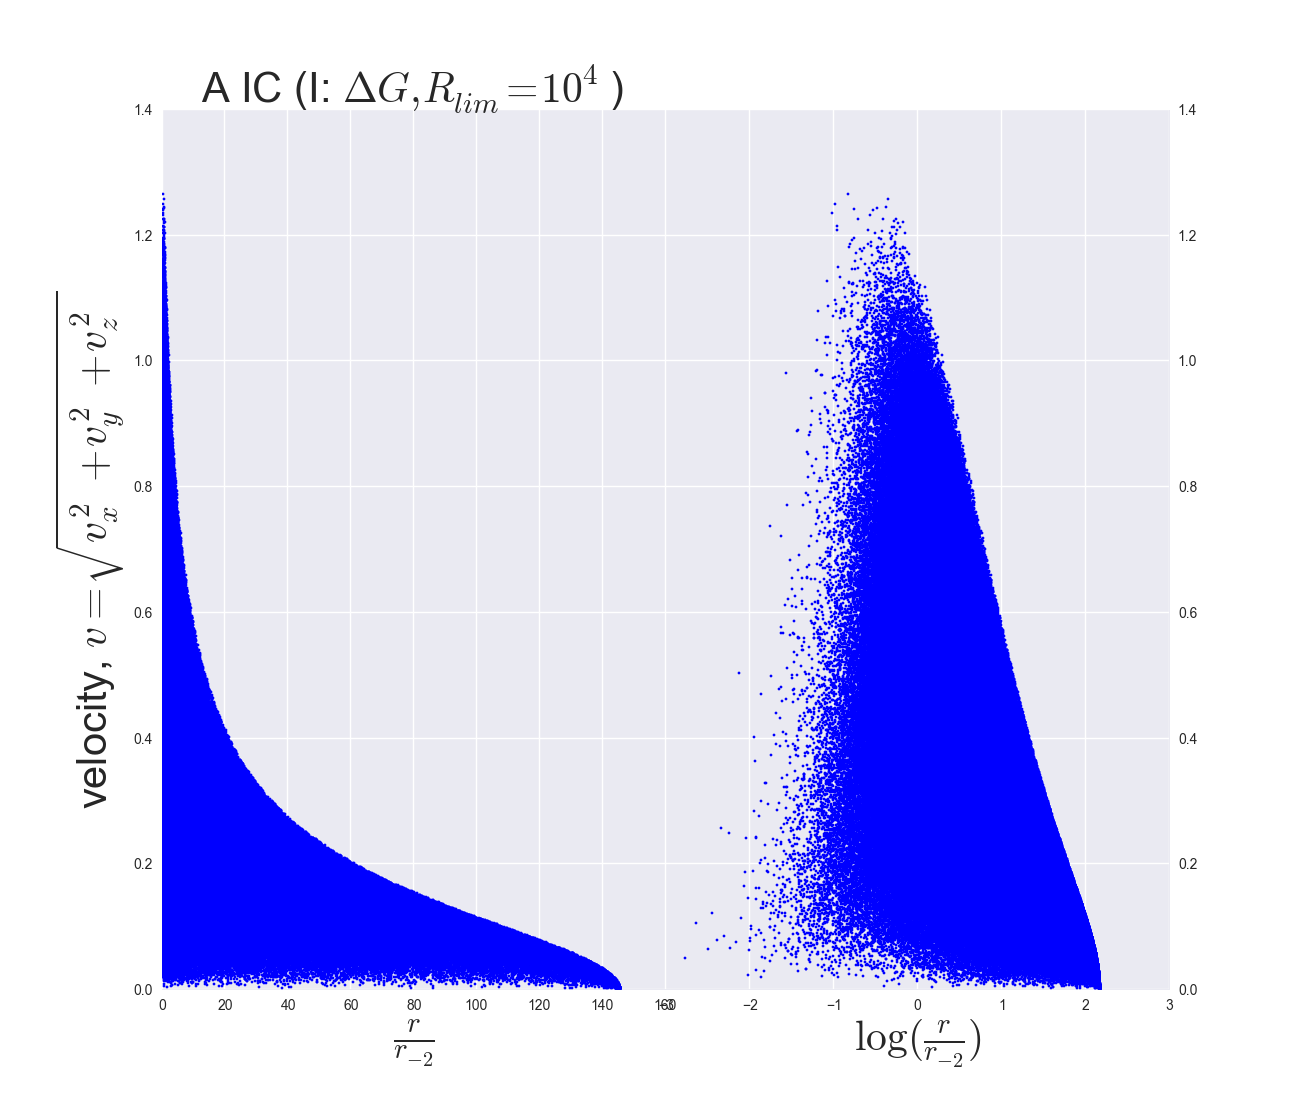
\includegraphics[width=1.0\linewidth]{img/A_IC_v_logr_r2.png}
\caption{Plot of $v_{tot}$ vs. $\frac{r}{r_{-2}}$ and $\log (\frac{r}{r_{-2}})$ respectively for IC of A. Analyzed out to a radius of $R_{lim} = 10^4$. Notice how the majority of particles are clustered around the value $\log (\frac{r}{r_{-2}}) = 0$.}
\label{fig:test}
\end{figure}

\begin{figure}[!htbp]
\centering
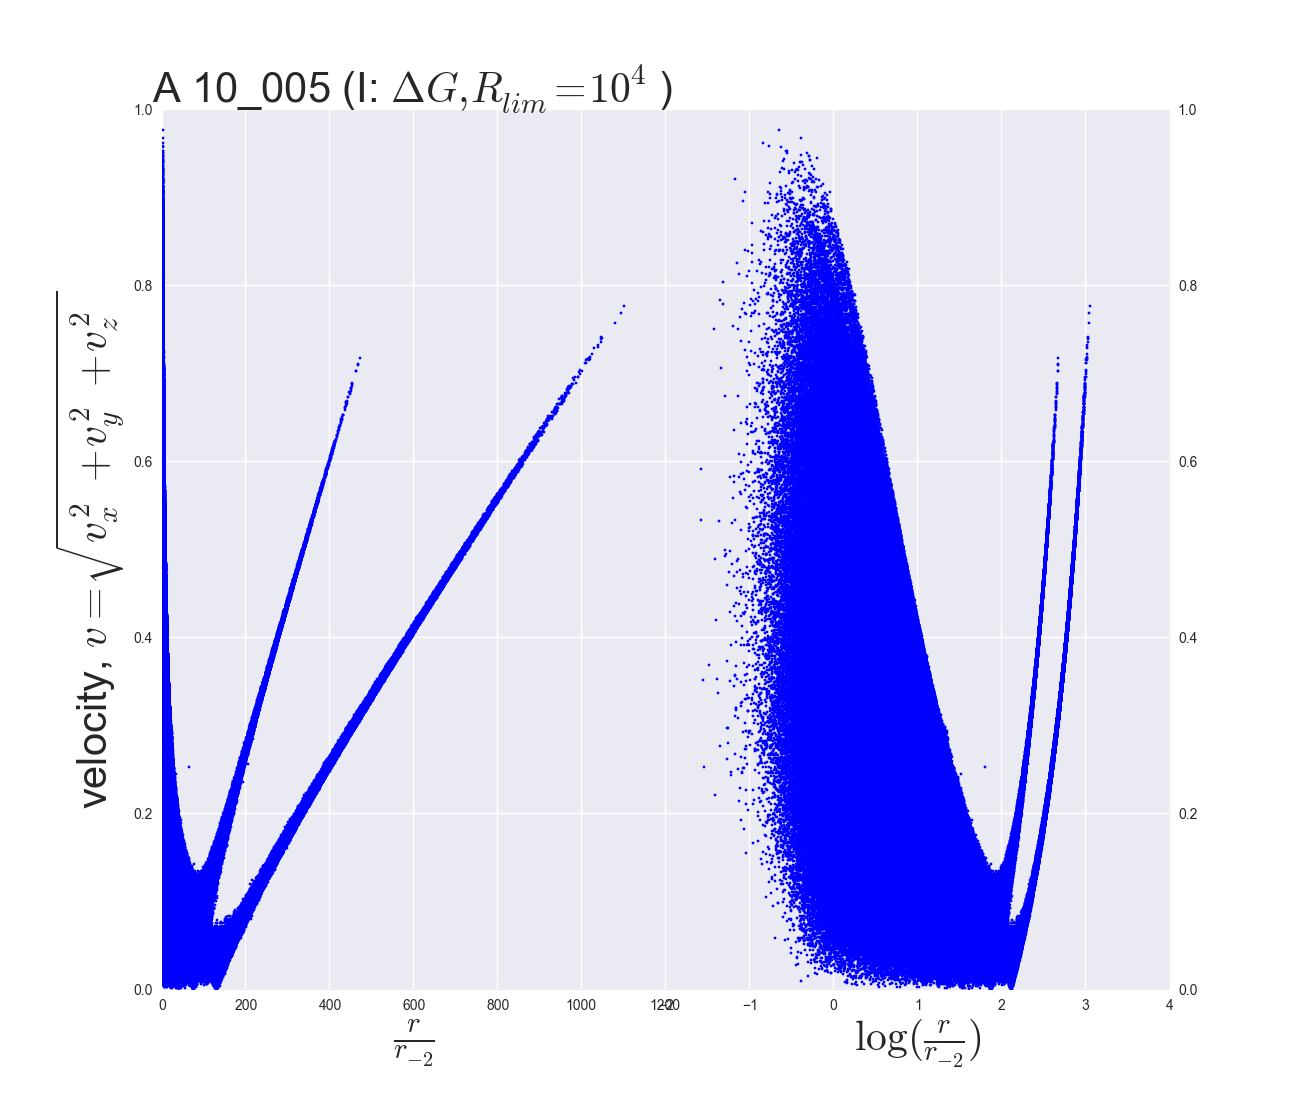
\includegraphics[width=1.0\linewidth]{img/A_10_005_v_logr_r2.png}
\caption{$v_{tot}$ vs. $\frac{r}{r_{-2}}$ and $\log (\frac{r}{r_{-2}})$ respectively for sim. I of structure A, after 1100 simulation timesteps (corresponding to $11\cdot t_{dyn}$ at $r=13.7\cdot r_s$). Analyzed out to a radius of $R_{lim} = 10^4$. A very slight shift of the main part of the structure towards larger radii is seen. Two velocity 'fingers' or velocity filaments can now be seen at larger radii. They are a direct response to the perturbation where $\Phi$ is first increased and then decreased due to a change in Newtons gravitational constant. This greatly increase particles velocities at large radii, forcing some of them to become gravitationally unbound. Two segments of 'G-chunks' have thus been run up to this stage as can be seen from simply counting the velocity filaments}
\label{fig:test}
\end{figure}

\begin{figure}[!htbp]
\centering
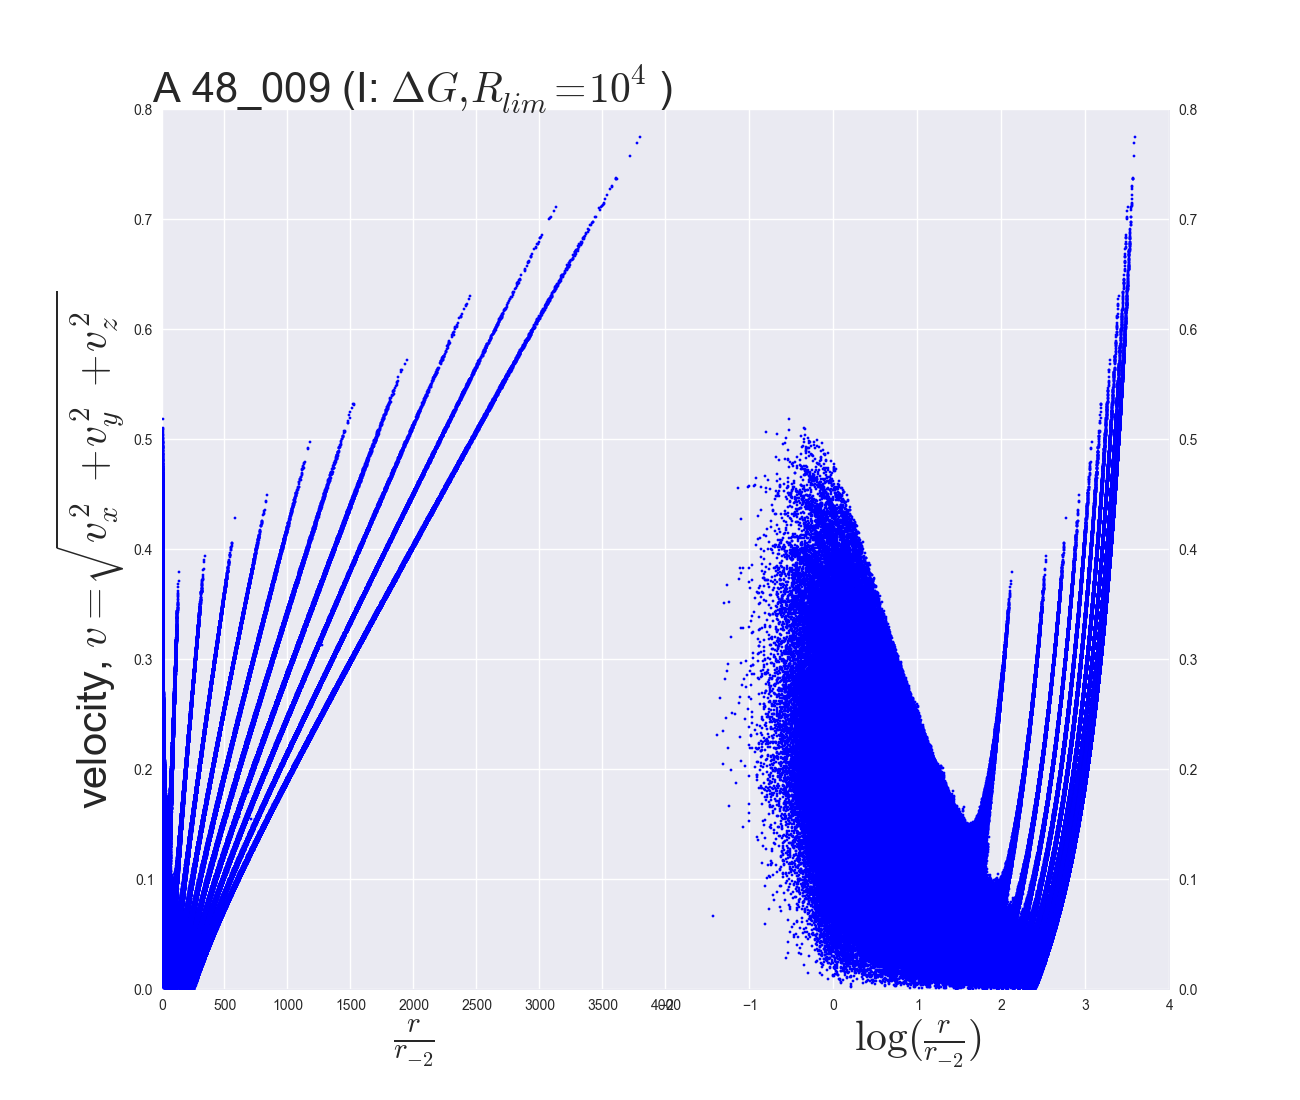
\includegraphics[width=1.0\linewidth]{img/A_48_009_v_logr_r2.png}
\caption{$v_{tot}$ vs. $\frac{r}{r_{-2}}$ and $\log (\frac{r}{r_{-2}})$ respectively for sim. I of structure A, after 4970 simulation timesteps (corresponding to $49.7\cdot t_{dyn}$ at $r=13.7\cdot r_s$). Analyzed out to a radius of $R_{lim} = 10^4$. The shifting of the main part of the structure towards larger radii remains present but is still not very significant. A much larger time span between this figure and the previous of $\Delta t_{sim} = 4970-1100 = 3870$ (or $38.7\cdot t_{dyn}$ at $r=13.7\cdot r_s$) means that far more 'G-chunks' have been run at this stage, in fact ten of them, and again counting the velocity filaments we see this to be illustrated by the existence of ten filaments.}
\label{fig:test}
\end{figure}

\begin{figure}[!htbp]
\centering
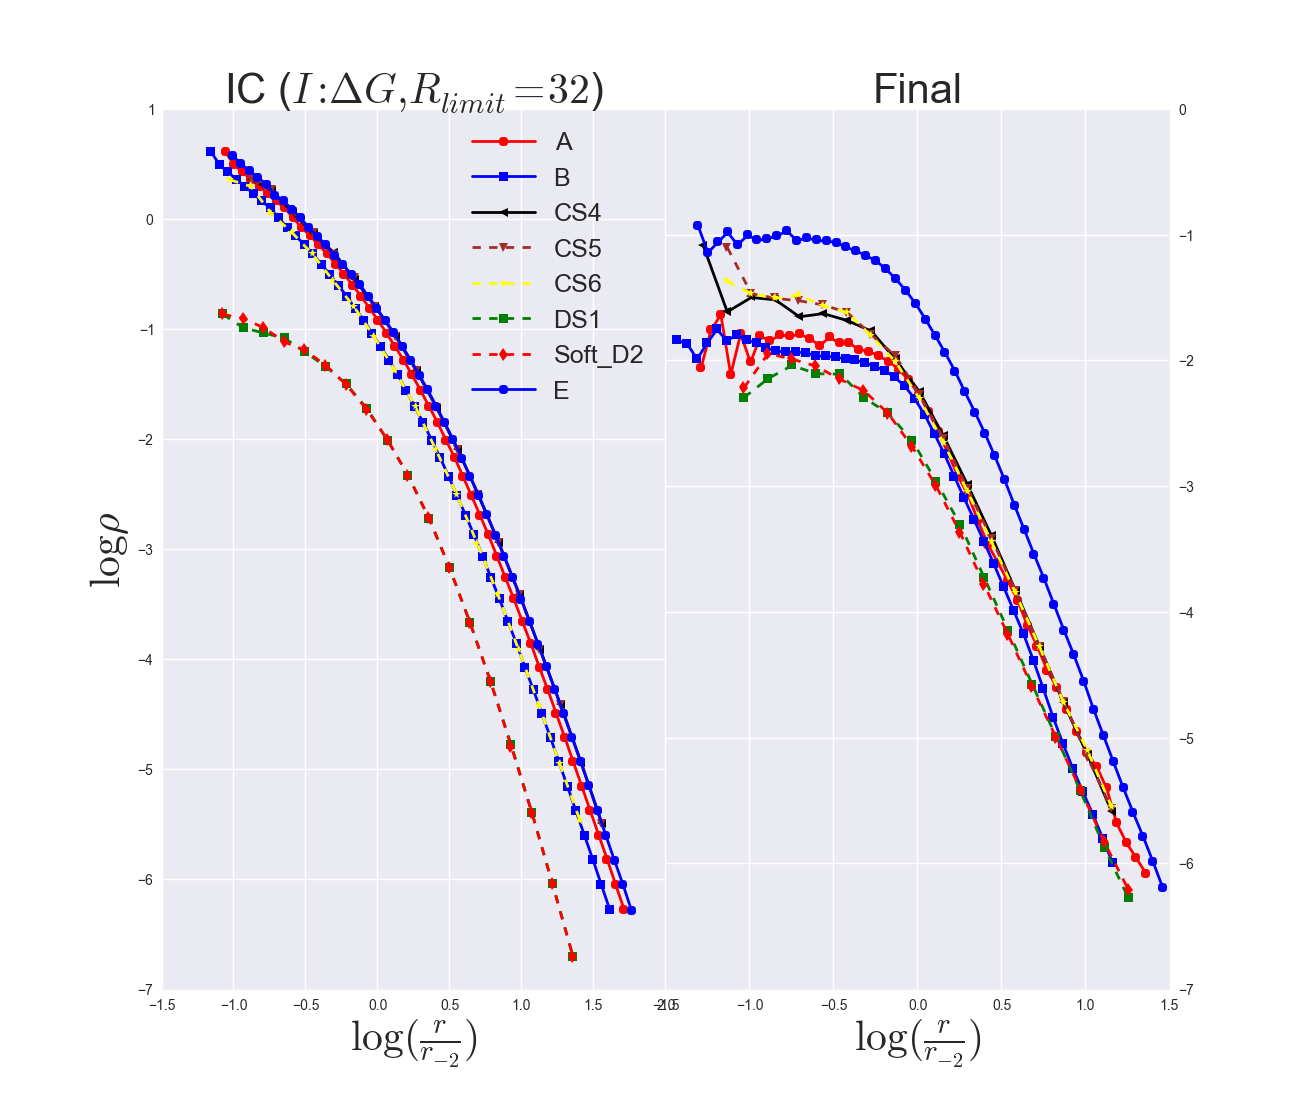
\includegraphics[width=1.0\linewidth]{img/log_r_r2_rho_IC_Final_R32.png}
\caption{$\rho$ vs. $\log (\frac{r}{r_{-2}})$. The IC profiles are all cuspy (apart from the DS1 and Soft$\_$D2 structures which have unique density profiles with inner and outer slope zero and minus 5 respectively); i.e. their inner density profiles are very steep. As time evolves all profiles develop small cores in the very inner region. This can be easily understood through some simple dynamical arguments; Consider the few central particles that just happens to have a very high velocity greater than the escape velocity of the halo. Increasing the gravitational potential and then letting the simulation run will make these central particles travel outwards as the now stronger potential will tend to on average pull the particles into, and through the center (as they do not experience any collisions). Once through the center their travel continues out to large radii from there they will move with constant speed away from the structure forever. Hence the catchphrase 'Once out, always out' applies to these high velocity central particles. This can be thought of as the main reason for the flattening of initially cuspy or steep density profiles at small radii. Structures with $N = 10^6$ particles (A, B and E) are divided into 50 bins which are logarithmic in radius, whereas structures with $N = 10^5$ particles are divided into just 20 bins to ensure a sufficient number of particles in each bin. The structures are cut off at a radius of $R_{lim} = 32\cdot r_s$ corresponding to the $log_{10}$ value of 1.5}
\label{fig:test}
\end{figure}

\begin{figure}[!htbp]
\centering
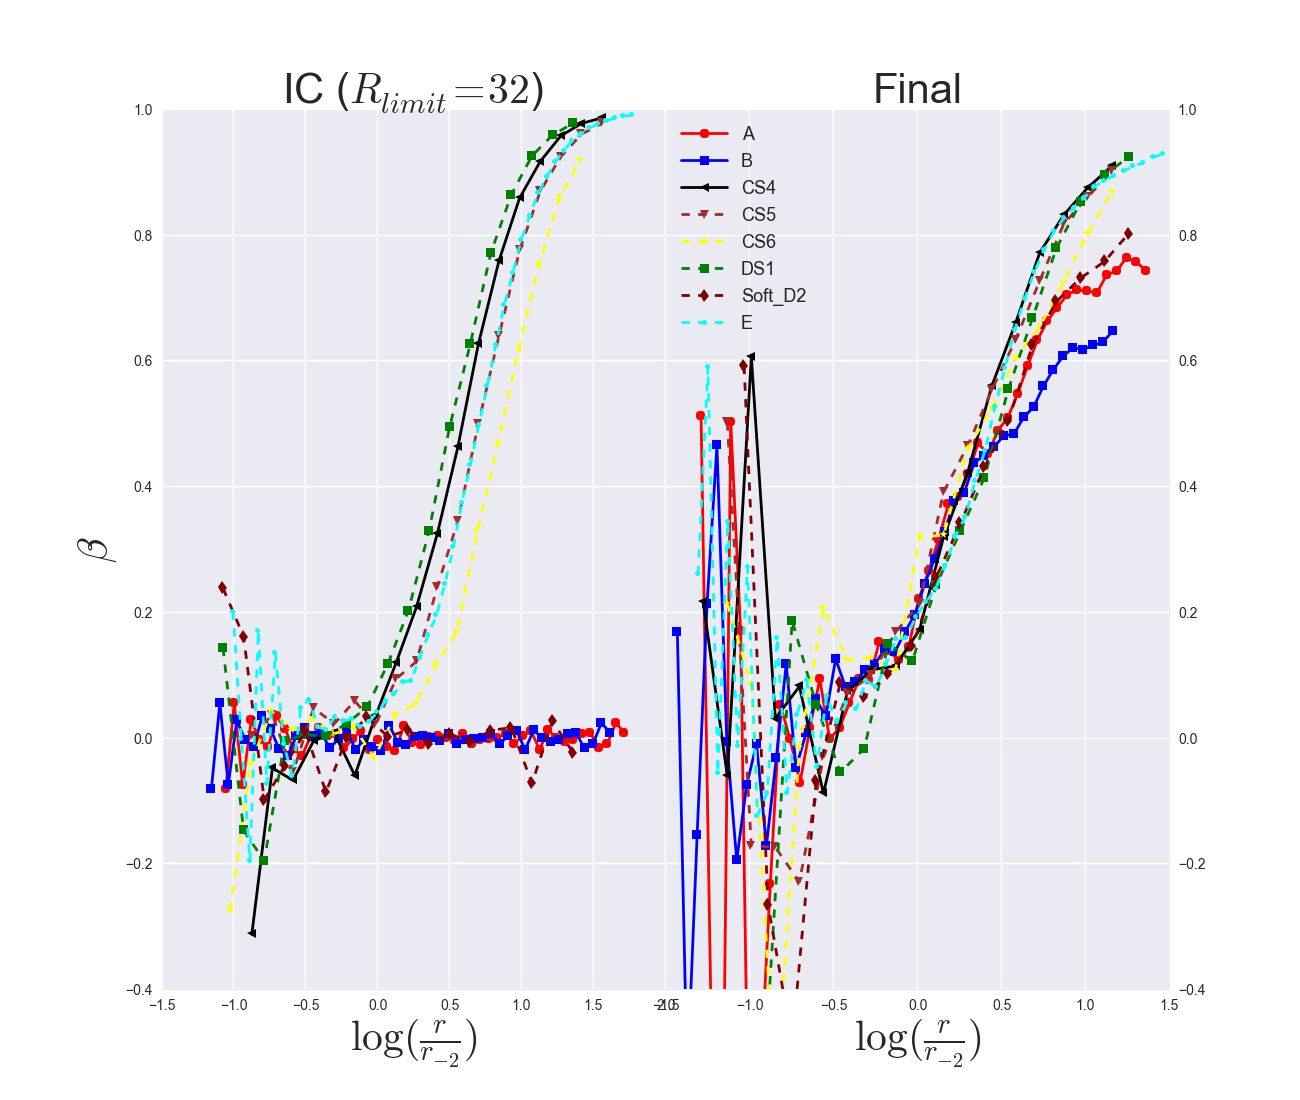
\includegraphics[width=1.0\linewidth]{img/Fig_logr_r2_beta_ABCS4CS5CS6DS1D2E_IC_Final_R_limit_32.png}
\caption{$\beta$ vs. $\log (\frac{r}{r_{-2}})$. By comparing IC with final products wrt the velocity anisotropy parameter $\beta$ it is seen that structures which are initially isotropic (A, B and Soft$\_$D2, created by Eddingtons inversion method) become radially biased over time and the structures with initial velocity anisotropy (CS4, CS5, CS6, DS1 and E, which are OM models) remain anisotropic in the outer part as time goes. The inner part of the final structures are dominated by large fluctuations due to Poisson noise and it is therefore not possible to say anything about this region for certain apart from the fact that the fluctuations are centered around $\beta = 0$ so the structures could be ergodic in the inner part. The span in the $\beta$ parameter for IC and final products are approximately $[-0.2;1.0]$, which can also be seen later in the ($\beta$,$\gamma$)- and ($\beta$,$\gamma + \kappa$)- plots. Structures with $N = 10^6$ particles (A, B and E) are divided into 50 bins which are logarithmic in radius, whereas structures with $N = 10^5$ particles are divided into just 20 bins to ensure a sufficient number of particles in each bin. The structures are cut off at a radius of $R_{lim} = 32\cdot r_s$ corresponding to the $log_{10}$ value of 1.5}
\label{fig:test}
\end{figure}

\begin{figure}[!htbp]
\centering
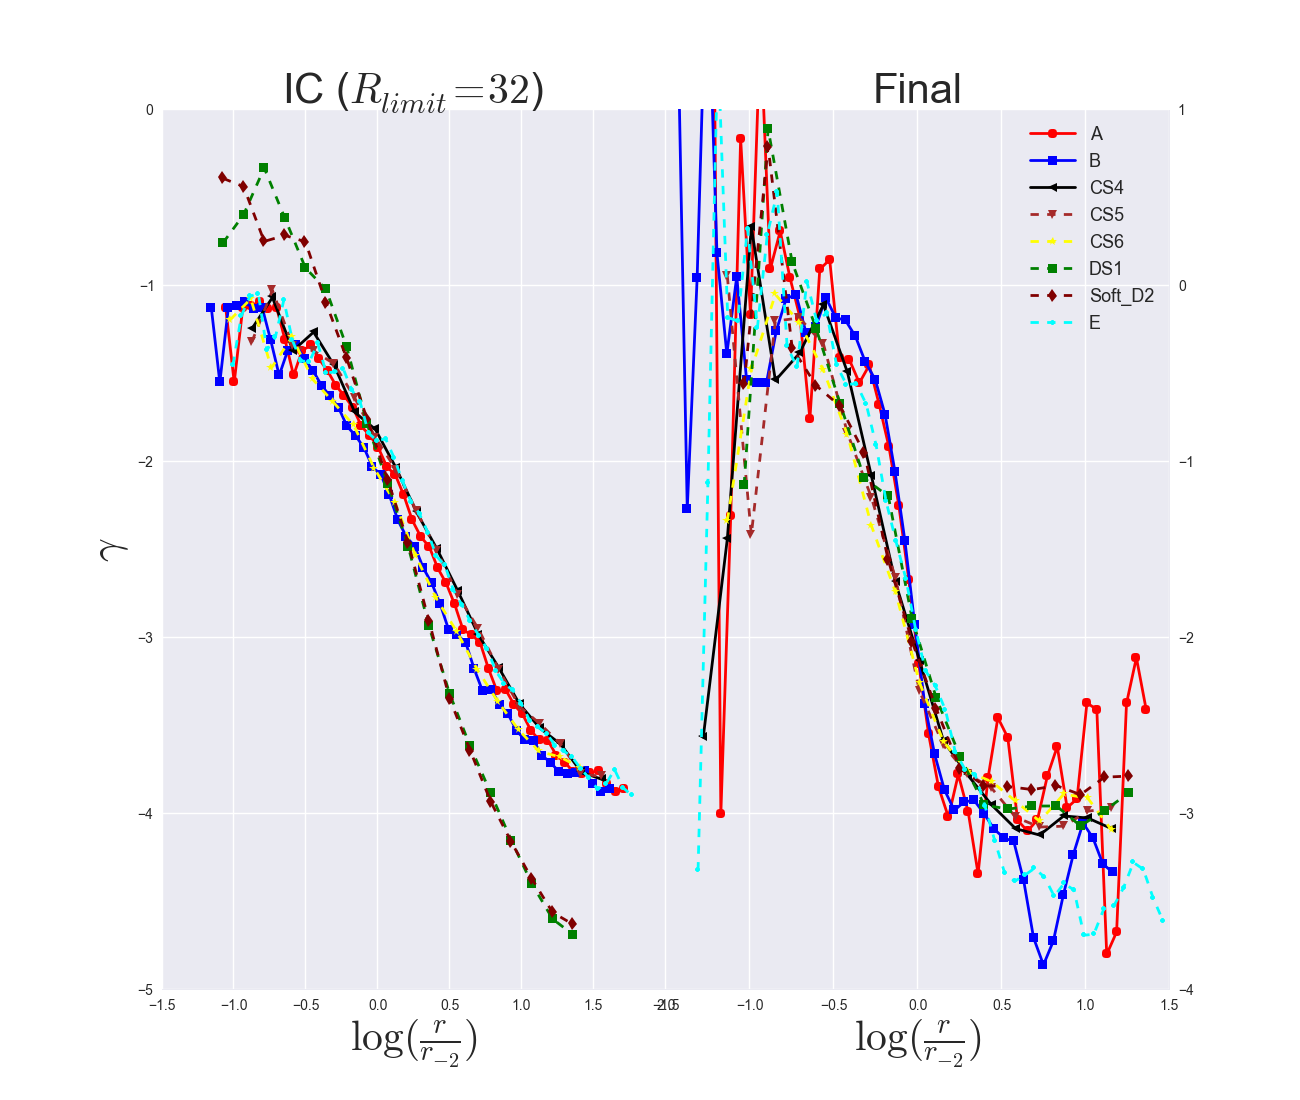
\includegraphics[width=1.0\linewidth]{img/Fig_logr_r2_gamma_ABCS4CS5CS6DS1D2E_IC_Final_R_limit_32.png}
\caption{$\gamma$ vs. $\log (\frac{r}{r_{-2}})$. Structures with $N = 10^6$ particles (A, B and E) are divided into 50 bins which are logarithmic in radius, whereas structures with $N = 10^5$ particles are divided into just 20 bins to ensure a sufficient number of particles in each bin. The structures are cut off at a radius of $R_{lim} = 32\cdot r_s$ corresponding to the $log_{10}$ value of 1.5}
\label{fig:test}
\end{figure}

\begin{figure}[!htbp]
\centering
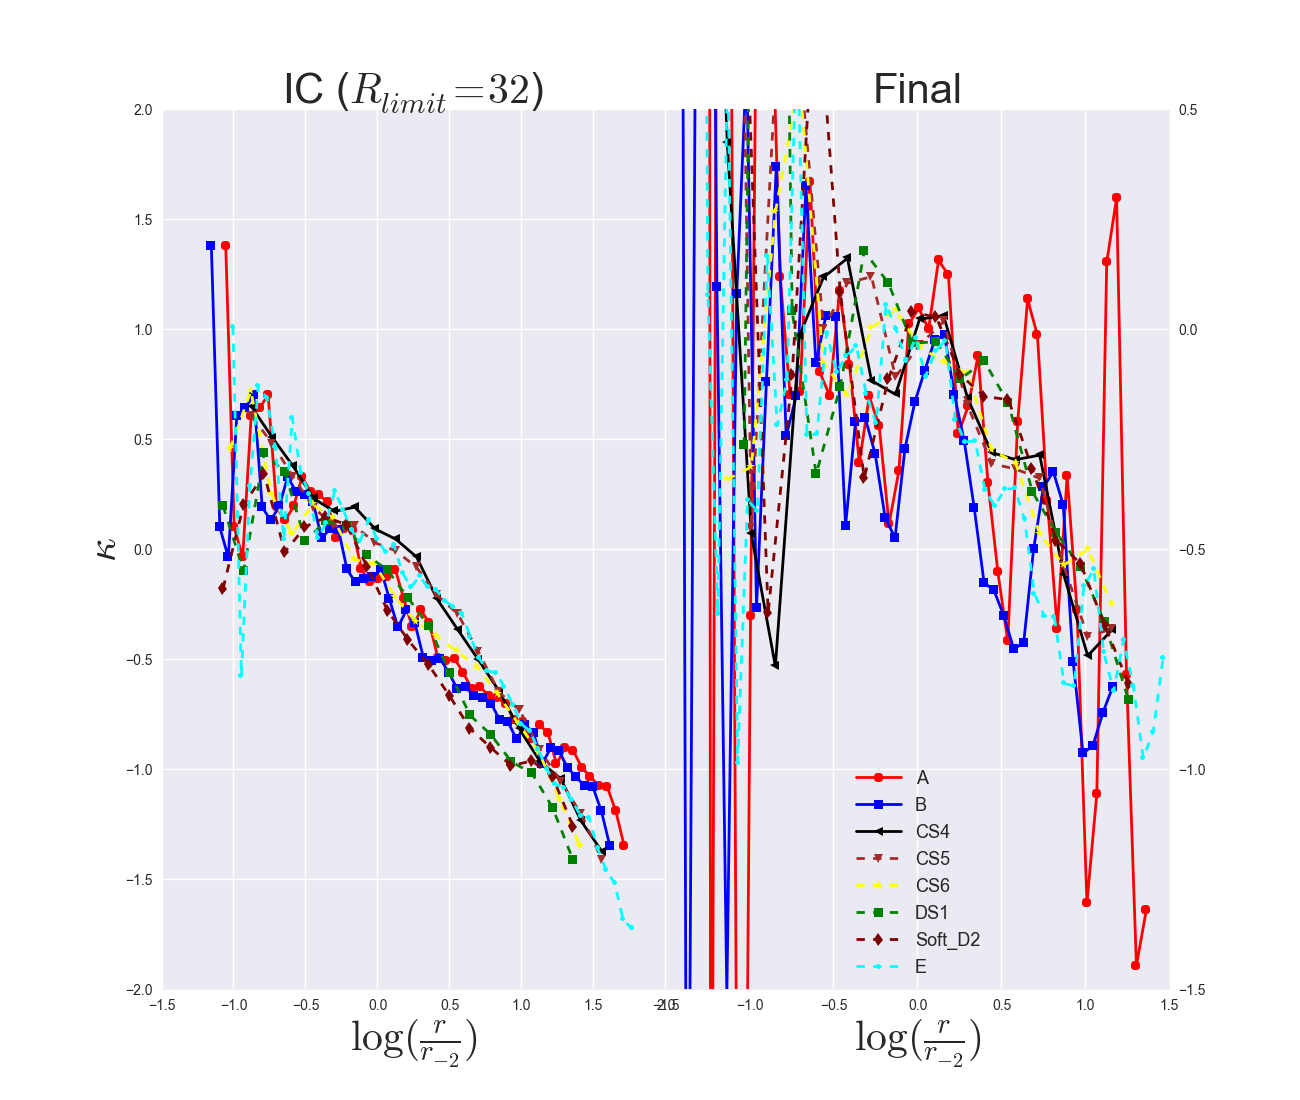
\includegraphics[width=1.0\linewidth]{img/Fig_logr_r2_kappa_ABCS4CS5CS6DS1D2E_IC_Final_R_limit_32.png}
\caption{$\kappa$ vs. $\log (\frac{r}{r_{-2}})$. Structures with $N = 10^6$ particles (A, B and E) are divided into 50 bins which are logarithmic in radius, whereas structures with $N = 10^5$ particles are divided into just 20 bins to ensure a sufficient number of particles in each bin. The structures are cut off at a radius of $R_{lim} = 32\cdot r_s$ corresponding to the $log_{10}$ value of 1.5}
\label{fig:test}
\end{figure}






\begin{figure}[!htbp]
\centering
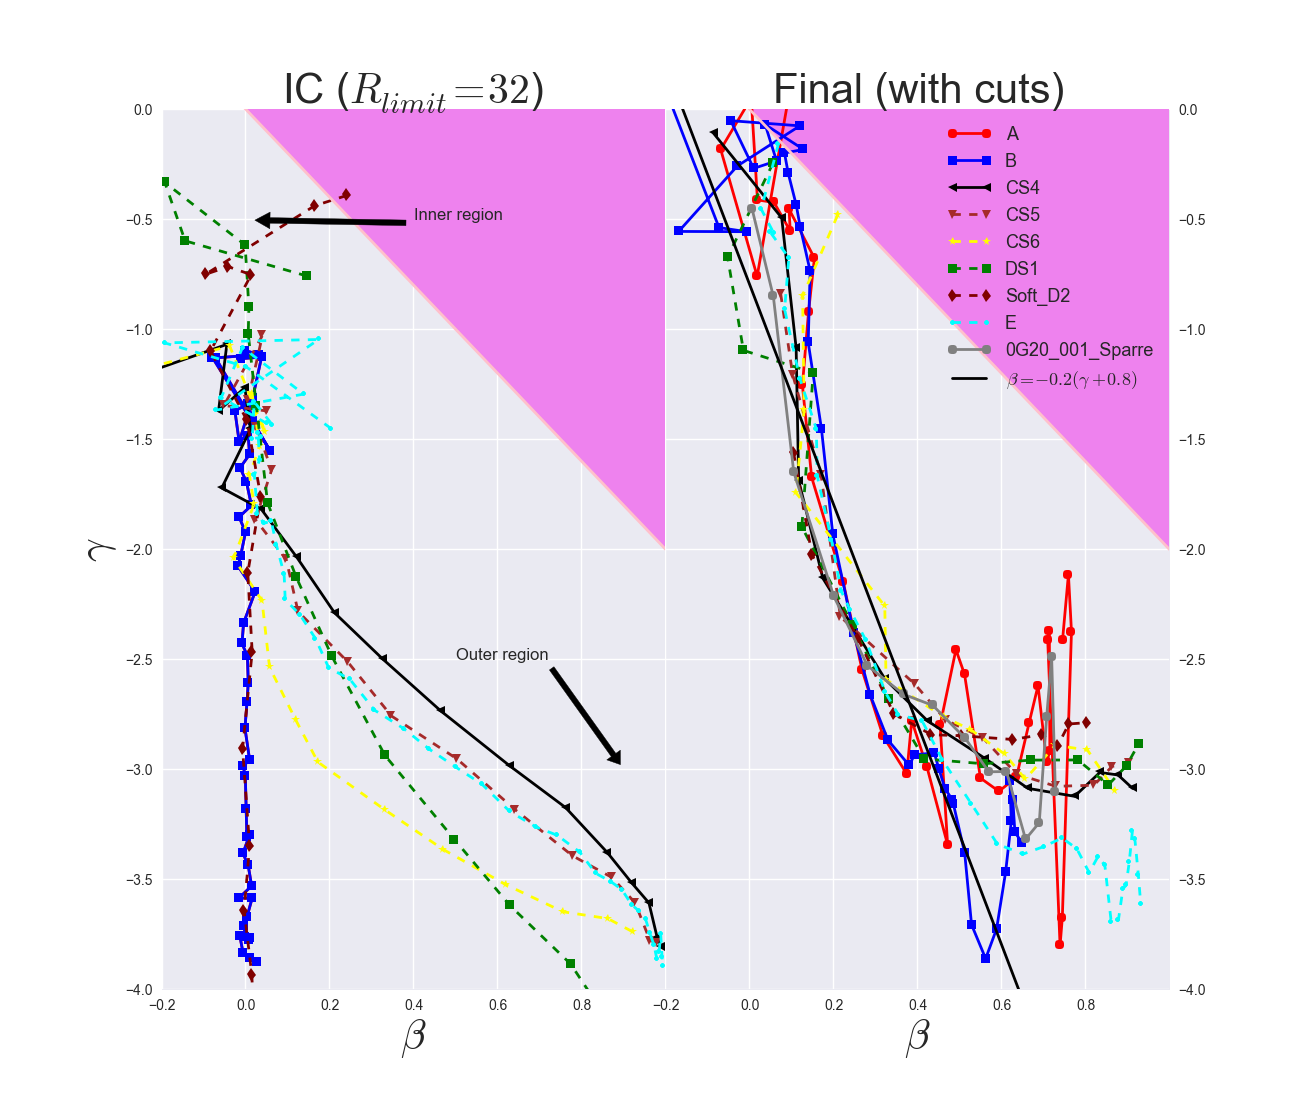
\includegraphics[width=1.0\linewidth]{img/Fig_beta_gamma_ABCS4CS5CS6DS1D2E_IC_Final_R_limit_32.png}
\caption{$\gamma$ vs. $\beta$. Left panel shows the initial conditions and right panel the final products after sim. I of structures A, B, $CS_4$, $CS_5$, $CS_6$, $DS_1$, $D_2$ and E. Notice how the IC spans a large volume of the Jeans parameter space whereas the final products are attracted to a 1-dimensional s-shaped attractor curve which effectively reproduces results found by others [4]. This attractor can be described analytically as $\gamma + \kappa = -8\beta $ for the inner part and $\gamma + \kappa = -0.7-4\beta $ for the outer region. For reference the final structures are plotted together with the linear relation found by Hansen and Moore (solid black line, $ \beta = -0.2(\gamma + 0.8)$) as well as data from [4] which are in very good agreement.}
\label{fig:test}
\end{figure}

\begin{figure}[!htbp]
\centering
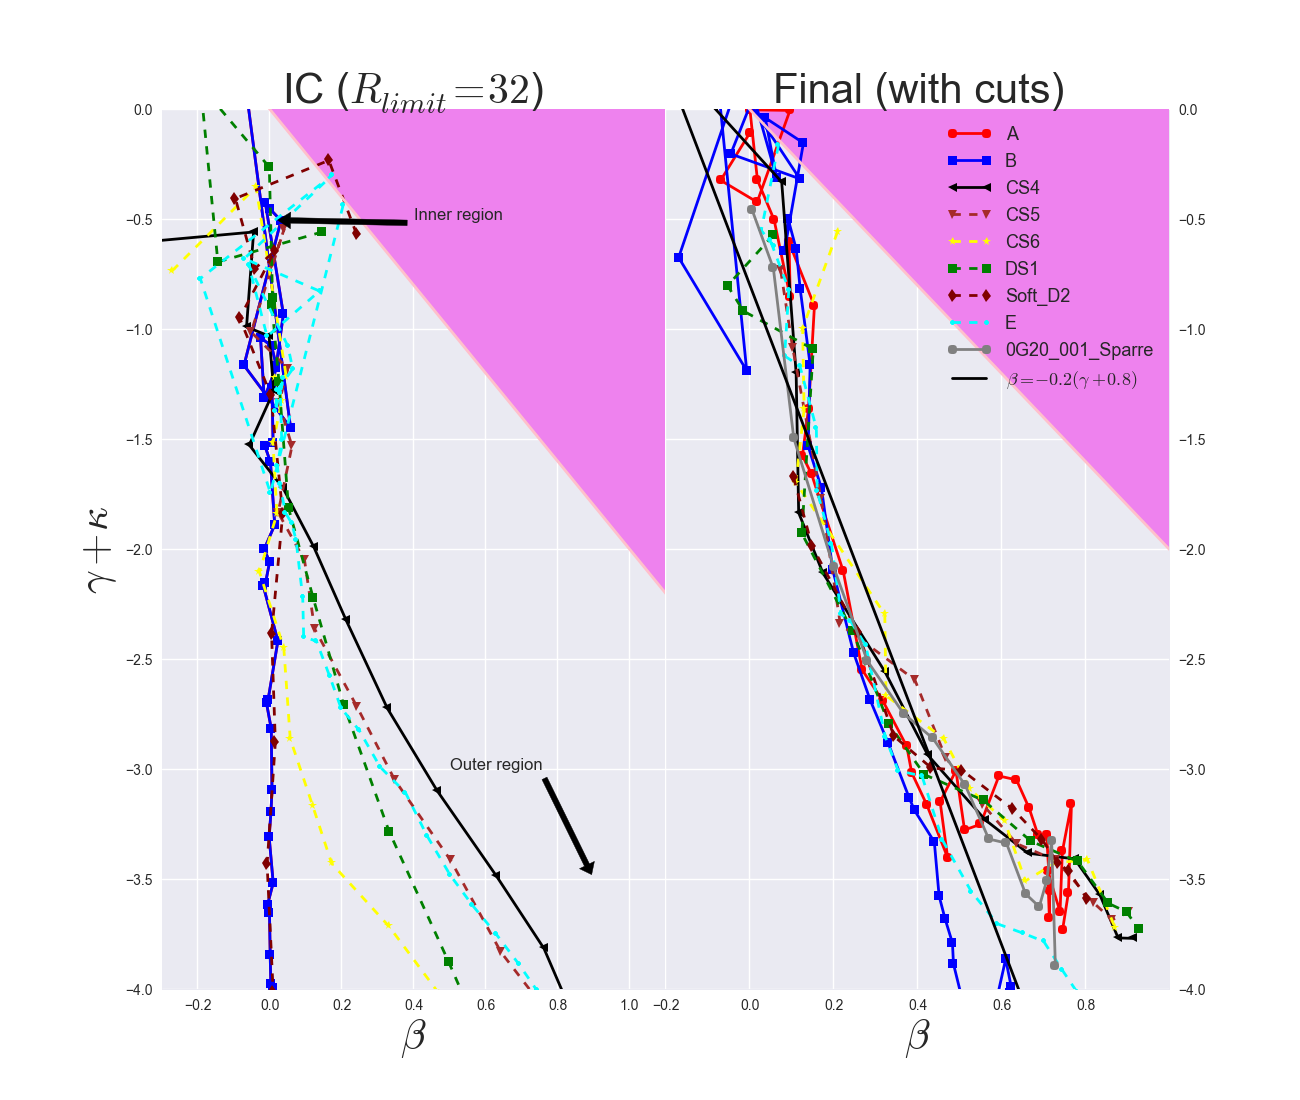
\includegraphics[width=1.0\linewidth]{img/Fig_beta_gamma_kappa_ABCS4CS5CS6DS1D2E_IC_Final_R_limit_32.png}
\caption{$\gamma + \kappa$ vs. $\beta$. Left panel shows the initial conditions and right panel the final products after sim. I of structures A, B, $CS_4$, $CS_5$, $CS_6$, $DS_1$, $D_2$ and E. Notice how the IC spans a large volume of the Jeans parameter space whereas the final products are attracted to a 1-dimensional s-shaped attractor curve which effectively reproduces results found by others [4]. This attractor can be described analytically as $\gamma + \kappa = -8\beta $ for the inner part and $\gamma + \kappa = -0.7-4\beta $ for the outer region. For reference the final structures are plotted together with the linear relation found by Hansen and Moore (solid black line, $ \beta = -0.2(\gamma + 0.8)$) as well as data from [4] which are in very good agreement.}
\label{fig:test}
\end{figure}

\subsubsection{IIa: Energy exchange (cartesian velocity perturbations)}
\textbf{Using structures holding a variety of initial conditions, this simulation type mimics effects found in galaxy mergers. Specifically, for all of these structures (named as $B$, $CS_4$, $CS_5$, $CS_6$, $DS_1$, $D_2$ and $E$) the total velocities inside spherical bins is perturbed for each of its particles by multiplying each of those given particles cartesian velocities ($v_x$, $v_y$ and $v_z$) by random numbers in different ranges, firstly the range $[0.8, 1.2]$ (corresponding to perturbing the kinetic energies by random numbers in the range $\frac{1}{2}\cdot[0.64, 1.44]$), taken from the continuous uniform distribution. This is a symmetric probability distribution where all intervals of the same length between 0.8 and 1.2 are equally probable. Following this exchange of kinetic energies between particles in fixed spherical bins, a normalization factor is applied to the total velocities, which ensures energy conservation. After such a velocity 'kick' the structures are simulated under their self gravity allowing them to flow a bit under their new velocities. This procedure is then repeated for a total of 40 runs (with one initial run where there is no perturbation. This allows the OM models to reach equilibrium, as they are not perfectly equilibrated when set up as OM models. It is done for Edd structures as well to be certain of equilibrium before any perturbations take effect). After the first 10 runs, the random number range is changed from $[0.8, 1.2]$ to $[0.95, 1.05]$ to look for more subtle effects in run 11 $\rightarrow$ 20. For run 21 $\rightarrow$ 40 the random range $[0.7, 1.3]$ is applied, and the runs 31 $\rightarrow$ 40 are given longer timespans to allow structures more flow (See table). This way of exchanging particle energies is reminiscent of phase mixing.} \\ \\

\begin{figure}[!htbp]
\centering
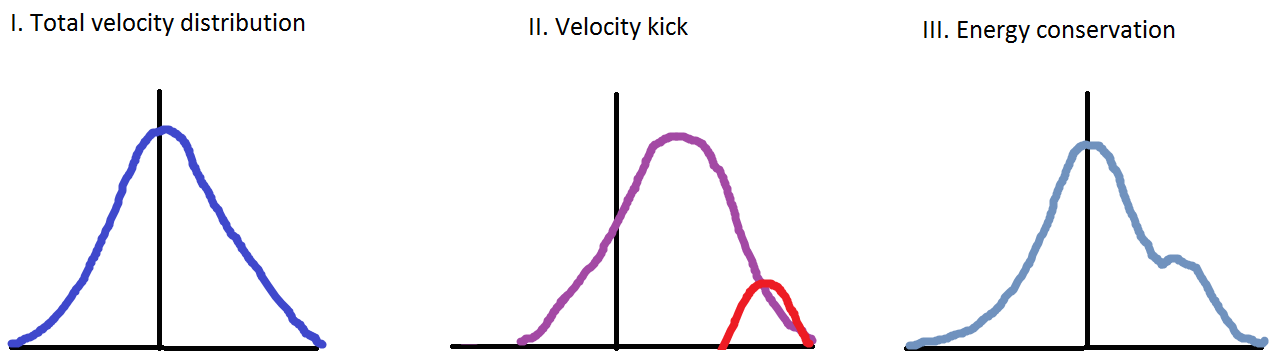
\includegraphics[width=15.0 cm]{img/Energy_exchange.png}
\caption{This simple cartoon illustrate the effects of the energy exchange simulation on the total velocity distribution. I: The initial distribution of the total velocity given in terms of cartesian coordinates,
$v=\sqrt{v_x^2+v_y^2+v_z^2}$. It follows a Gaussian shape with mean velocity equal to zero. \\
II: Velocity kicks are now given to each particle in the structure, by multiplication of the initial velocities with a uniformly distributed random number in the range [0.8, 1.2]. This has the effect of shifting the mean of the distribution towards higher values. Furthermore, some of the particles with very high velocities (and further away from the structures center, where the potential is weaker) now become gravitationally unbound. This is illustrated by the red bump at the right tail of the right-shifted, randomized velocity curve shown in purple. The total energy is now higher than what it was initially. As the velocities were perturbed by factors in the range [0.8, 1.2], the kinetic energies $K \propto v^2$ will have their initial values changed by factors in the range [0.64, 1.44] giving a new kinetic energy span of [1-0.36, 1+1.44] times the initial kinetic energies.\\
III: In order to conserve energy, a normalization factor is multiplied with the initial energy, and used to normalize particle velocities after the previous randomization, so that the velocity mean of zero is regained. A small bump at the right tail remains however, which is seen on the final curve shown in pale blue.}
\label{fig:test}
\end{figure}

\begin{table}[!htbp]
\centering
\begin{tabular}{|c|c|c|}
 \hline
 Run No. & velocity kicks &  Flow time  \\ \hline
   0     &     0 $\%$     &     100     \\ \hline
 1-10    &    20 $\%$     &     100     \\ \hline
 11-20	 &     5 $\%$     &     100     \\ \hline
 21-30	 &    30 $\%$     &     100     \\ \hline
 31-40	 &    30 $\%$     &     500     \\ \hline
\end{tabular}
\caption {Simulation II pattern. The left column shows the number of run in question. 
The middle column gives the maximum percentage of velocity kick to each particle along each of the three cartesian velocity directions, $v_x$, $v_y$ and $v_z$. Finally the right column states the time allowed for structures to flow freely under their self gravity. Run 0 takes place without any prior perturbation and lasts for 100 simulation times. In short, all structures are given medium velocity kicks before the first 10 runs following perturbations (run 1 $\rightarrow$ 10), while they are given small kicks before run 11 $\rightarrow$ 20, large kicks are given for run 21 $\rightarrow$ 40. Each of the runs from 1 $\rightarrow$ 30 lasts for 100 simulation times, but the last 10 runs (31 $\rightarrow$ 40) are given 500 simulation times each.}
\end{table}

This whole process of velocity-kick and energy normalization is followed by a phase of flow after which the pattern is repeated (kick $\rightarrow$ flow). A parallel control simulation (with 20 runs) is performed where the energy is not exchanged in this manner. No alterations are done; i.e. G remains at unity throughout and no velocity kicks are given by hand to any particle. The purpose of this control simulation is to make sure the structures stay in equilibrium and provide a means of comparison for the perturbed structures. 
Binning of structures is done in the following way:
First the radius of all particles to the halo center is sorted from smallest to largest value and this sorting is then applied to the positions and velocities as well as the potential. Now number bins are created so that each bin holds exactly 500 particles and runs from smallest to largest radii. The volume of each bin is hence generally different and depends on the mean inter-particle distance which grows as radius increases. It is therefore the case that outermost bins take up more space than innermost number-bins. Inside each number bin the perturbation and normalizing of particle velocities and energies can then be performed. Finally saving the perturbed structures into a new snapshotfile, this is then ready to be read and simulated by the GADGET-2 code. More specifically about the perturbations:
Starting out by giving each particle a velocity kick by a random number in the above stated range for each of its three cartesian velocity directions provide the particles with a new velocity given by 

\centerline{$v_{rand} = \sqrt{v_{x,rand}^2 + v_{y,rand}^2 + v_{z,rand}^2}$}

where for example 

\centerline{$v_{z,rand} = v_z^{initial} + \Delta v_z = v_z^{initial}\big( 1 + rand[0.8,1.2] \big) $}

and 	$rand[0.8,1.2]$ is a uniform random number between 0.8 and 1.2, thus perturbing each of the cartesian velocity components by maximally 20 \% which in turn means that the maximum perturbation to the total velocity vector can be $\sqrt{1200} \% = 20\cdot \sqrt{3} \% \approx 34.6 \%$.
The kinetic energy becomes 

\centerline{$K_{rand}=\frac{1}{2}v_{rand}^2$}

In order to ensure energy conservation normalization factors must be multiplied to the new velocities.
The particles are split into gravitationally bound (where $\Phi + K \leq 0 $) and unbound (where $\Phi + K > 0 $). The unbound particles new velocities are first multiplied by a random number in the range $[0.8, 1.0]$ and subsequently normalized by multiplying them with 

\centerline{$ \sqrt{\frac{ \sum |\Phi|}{ \sum K_{rand}}}$} 

After this normalization the kinetic energy is determined as 

\centerline{$K_{rand, norm}=\frac{1}{2}v_{new}^2$,} 

where $v_{new}$ is the concatenation of initially bound, and the now bound particles (after normalization).
Then the new cartesian velocities are normalized by multiplying them with 

\centerline{$ \sqrt{\frac{<K_{initial}>}{<K_{rand, norm}>}}$,} 

where $<K_{initial}>$ and $<K_{rand, norm}>$ are the kinetic energies initially and after randomization plus normalizations, respectively. This gives the final velocities 

\centerline{$v_{final} = \sqrt{v_{x,final}^2 + v_{y,final}^2 + v_{z,final}^2}$}

Now the kinetic energy is $K_{final}=\frac{1}{2}v_{final}^2$ and the average value equals the average of the initial kinetic energy.

\begin{figure}[!htbp]
\centering
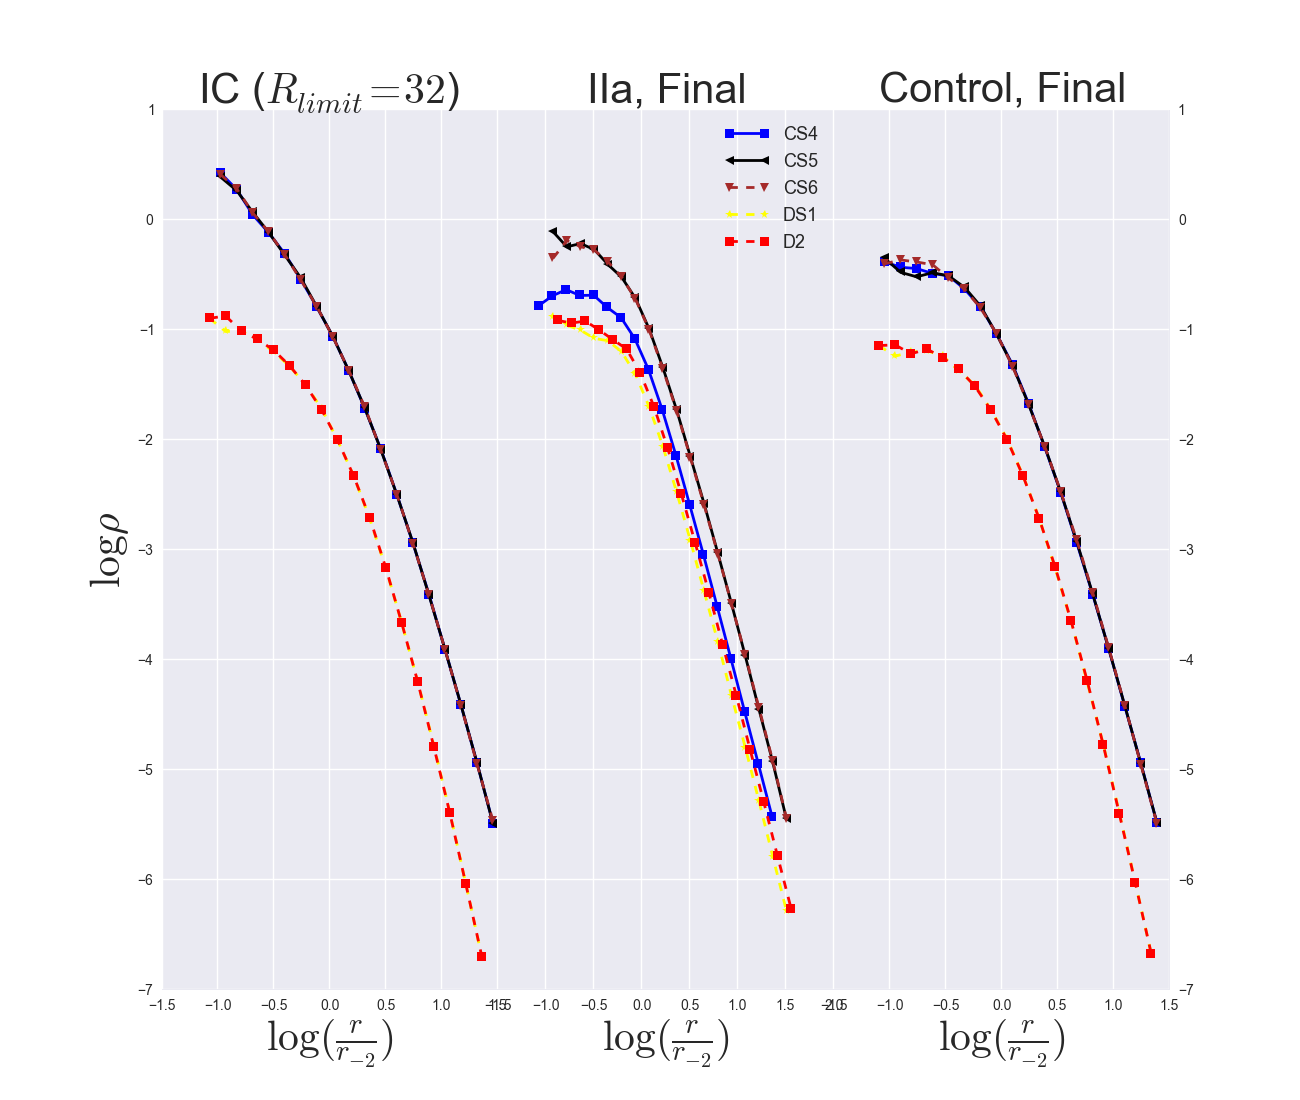
\includegraphics[width=1.0\linewidth]{img/logr_logrho.png}
\caption{Density profiles. $\log (\rho)$ vs. $\log \frac{r}{r_{-2}}$ for Sim. IIa of stable structures $CS_4$, $CS_5$, $CS_6$, $DS_1$ and $D_2$. First subplot from the left shows the IC's, middle subplot shows final products and right subplot shows final products of the control runs where no perturbations were applied to any of the structures. The right subplot thus serves as a efficient means of comparison with the final products of Sim. IIa. The formation of a core is seen for the final products as time evolves. 20 radial bins is used for these structures which have $N = 10^5$ particles.}
\label{fig:test}
\end{figure}

\begin{figure}[!htbp]
\centering
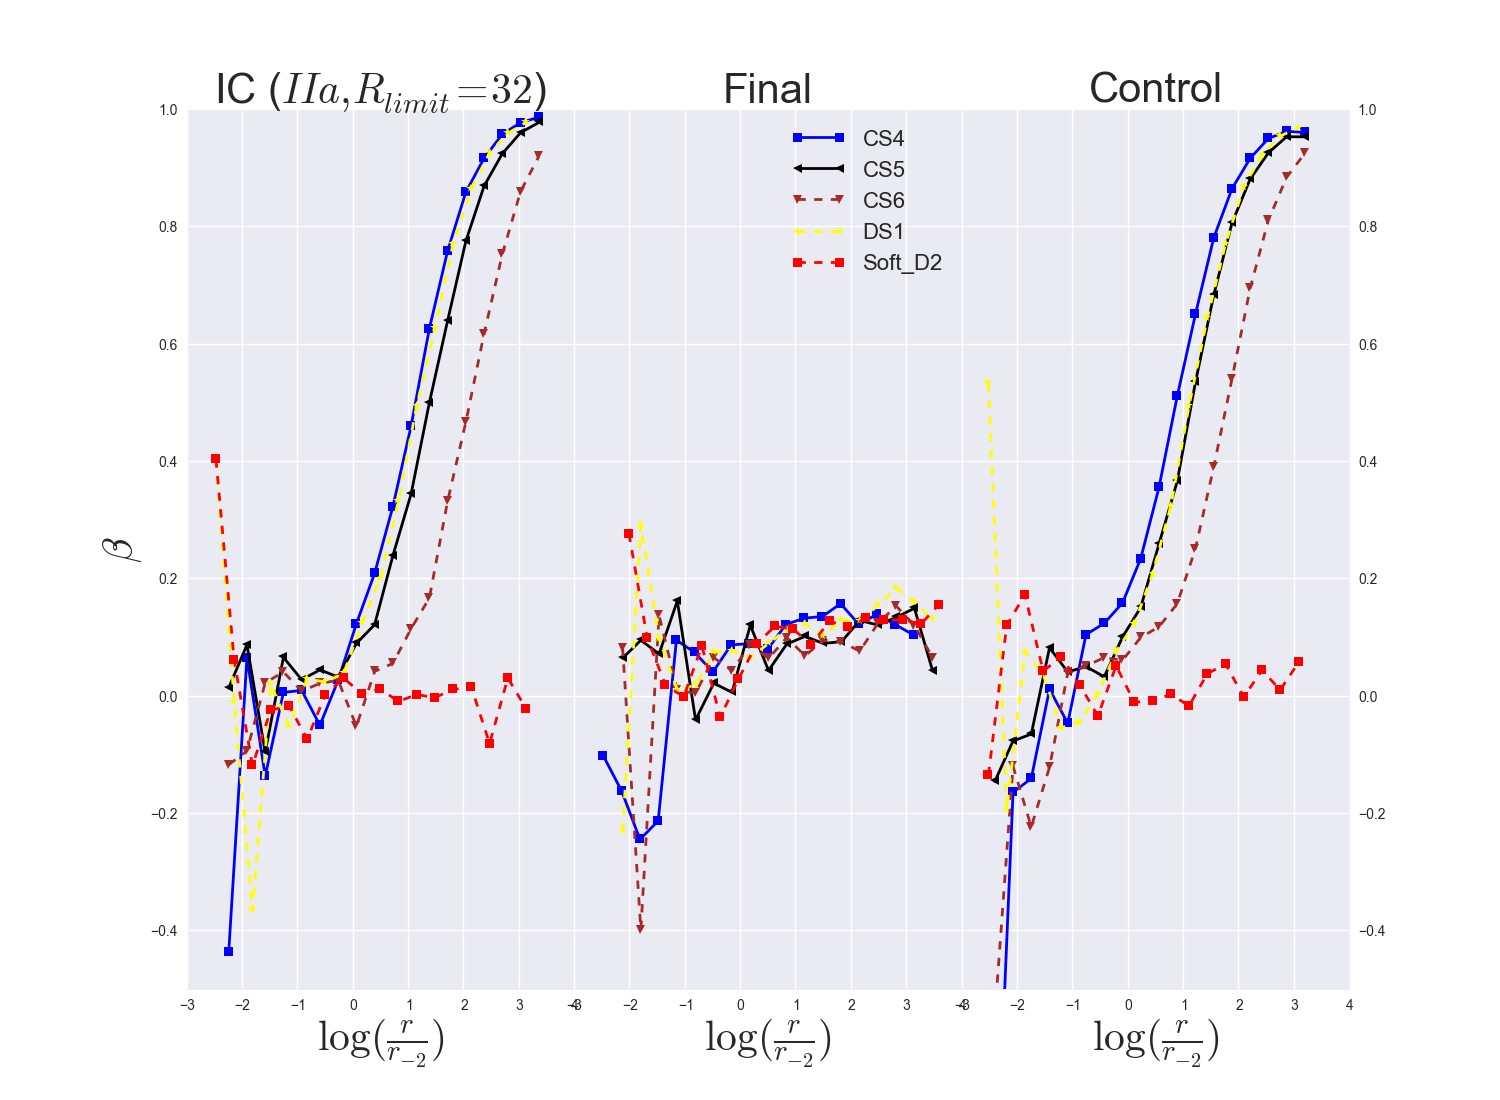
\includegraphics[width=1.0 cm]{img/log_r_r2_beta_CS4CS5CS6DS1D2_Rlimit32.png}
\caption{$\beta$ profiles for Sim. IIa of stable structures $CS_4$, $CS_5$, $CS_6$, $DS_1$ and $D_2$.
Structures are cut off at a radius of 32 times the scale radius. 20 radial bins are used. 
Initial conditions with either complete velocity isotropy or slightly anisotropic ones are both seen to be driven towards a new attractor
in the outer regions where they tend to land close to $\beta = 0.1$ (see middle panel).
The control runs which are simulated with no perturbations interfering can be seen in the right panel.
They show no significant departure from the initial conditions shown in the left panel.}
\label{fig:test}
\end{figure}

\begin{figure}[!htbp]
\centering
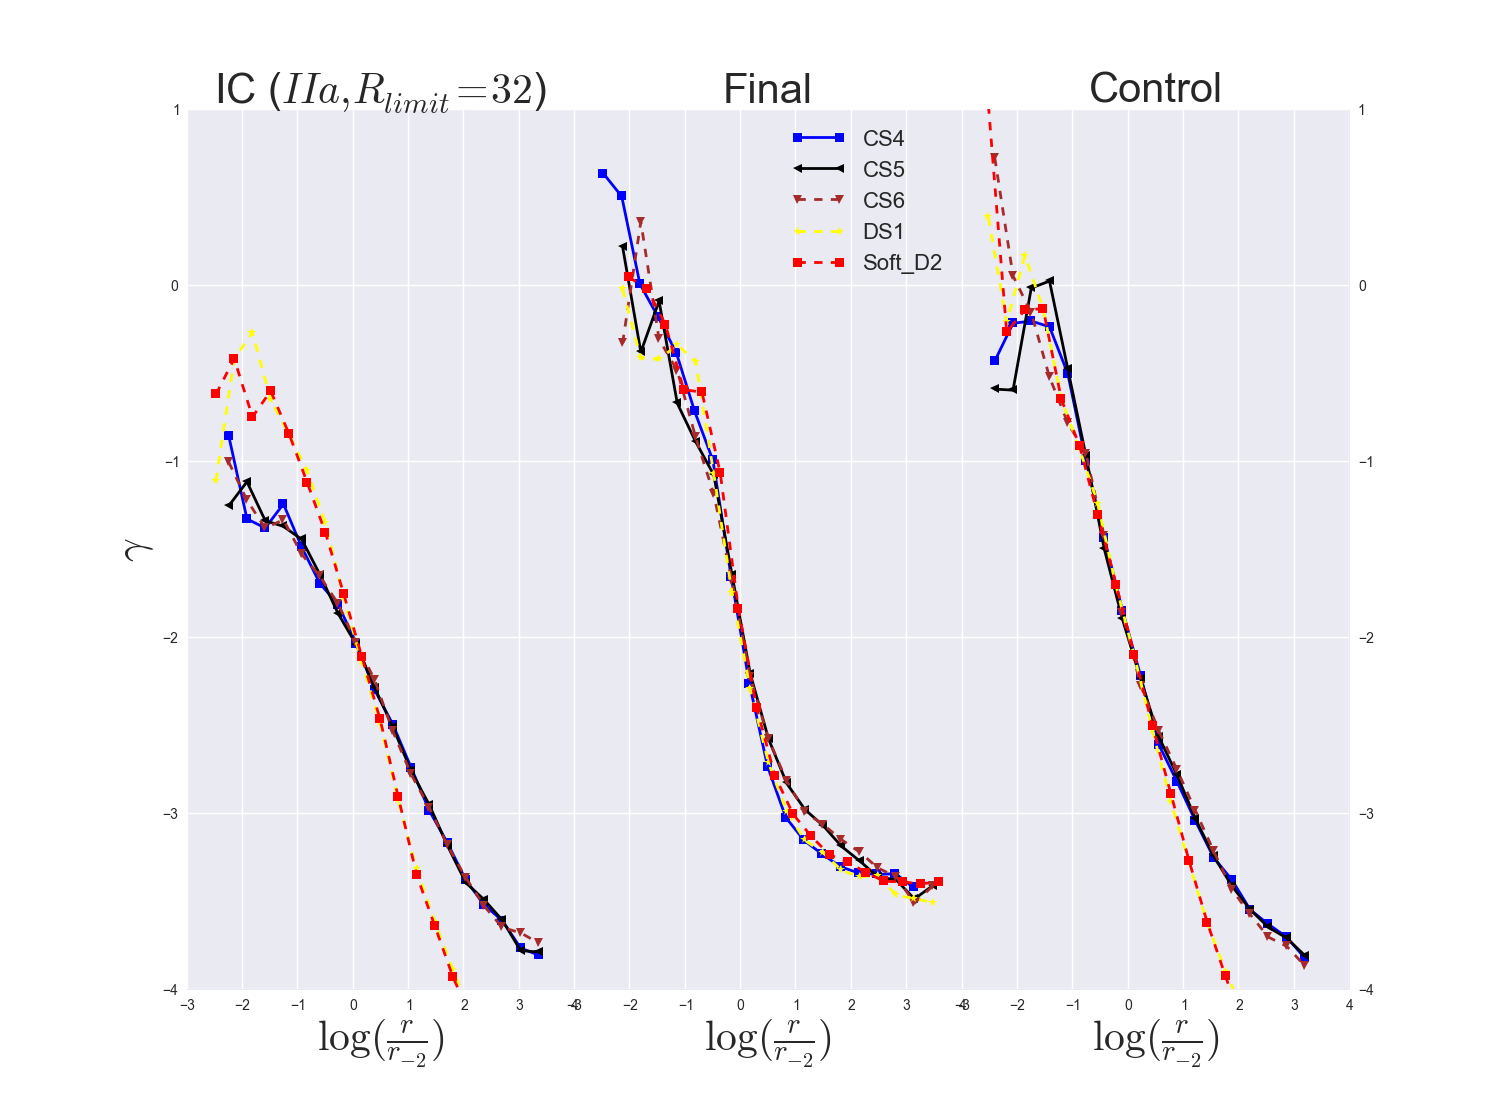
\includegraphics[width=1.0 cm]{img/log_r_r2_gamma_CS4CS5CS6DS1D2_Rlimit32.png}
\caption{$\gamma$ profiles for Sim. IIa of stable structures $CS_4$, $CS_5$, $CS_6$, $DS_1$ and $D_2$.
Structures are cut off at a radius of 32 times the scale radius. 20 radial bins are used. 
The final structures in the middle panel can be seen to get attracted towards a characteristic curve.
The $\gamma$ profiles thus have a preferred structure as very different initial conditions all flow towards this configuration.
The control runs which are simulated with no perturbations interfering can be seen in the right panel.
They show no significant departure from the initial conditions shown in the left panel.}
\label{fig:test}
\end{figure}

\begin{figure}[!htbp]
\centering
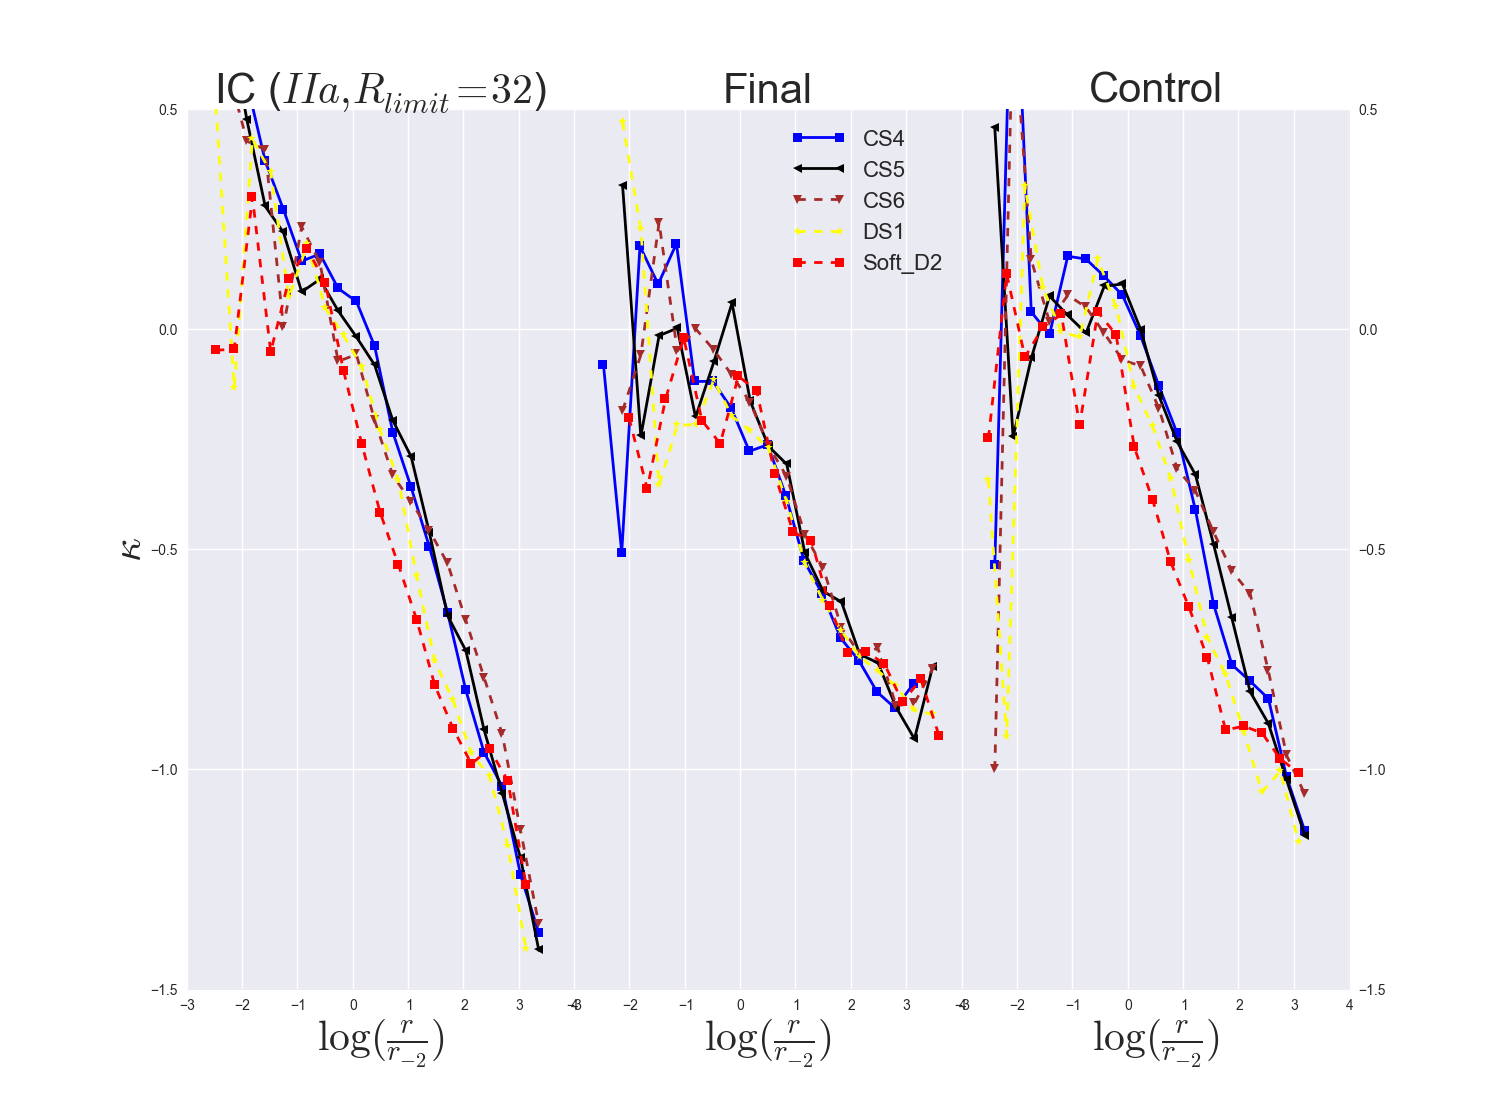
\includegraphics[width=1.0 cm]{img/log_r_r2_kappa_CS4CS5CS6DS1D2_Rlimit32.png}
\caption{$\kappa$ profiles for Sim. IIa of stable structures $CS_4$, $CS_5$, $CS_6$, $DS_1$ and $D_2$.
Structures are cut off at a radius of 32 times the scale radius. 20 radial bins are used. 
The middle panel reveals an attractor for the end products wrt. the $\kappa$-profiles.
This attractor is present for $\log \frac{r}{r_{-2}} > 0.5$. 
The control runs which are simulated with no perturbations interfering can be seen in the right panel.
They show no significant departure from the initial conditions shown in the left panel.}
\label{fig:test}
\end{figure}

\begin{figure}[!htbp]
\centering
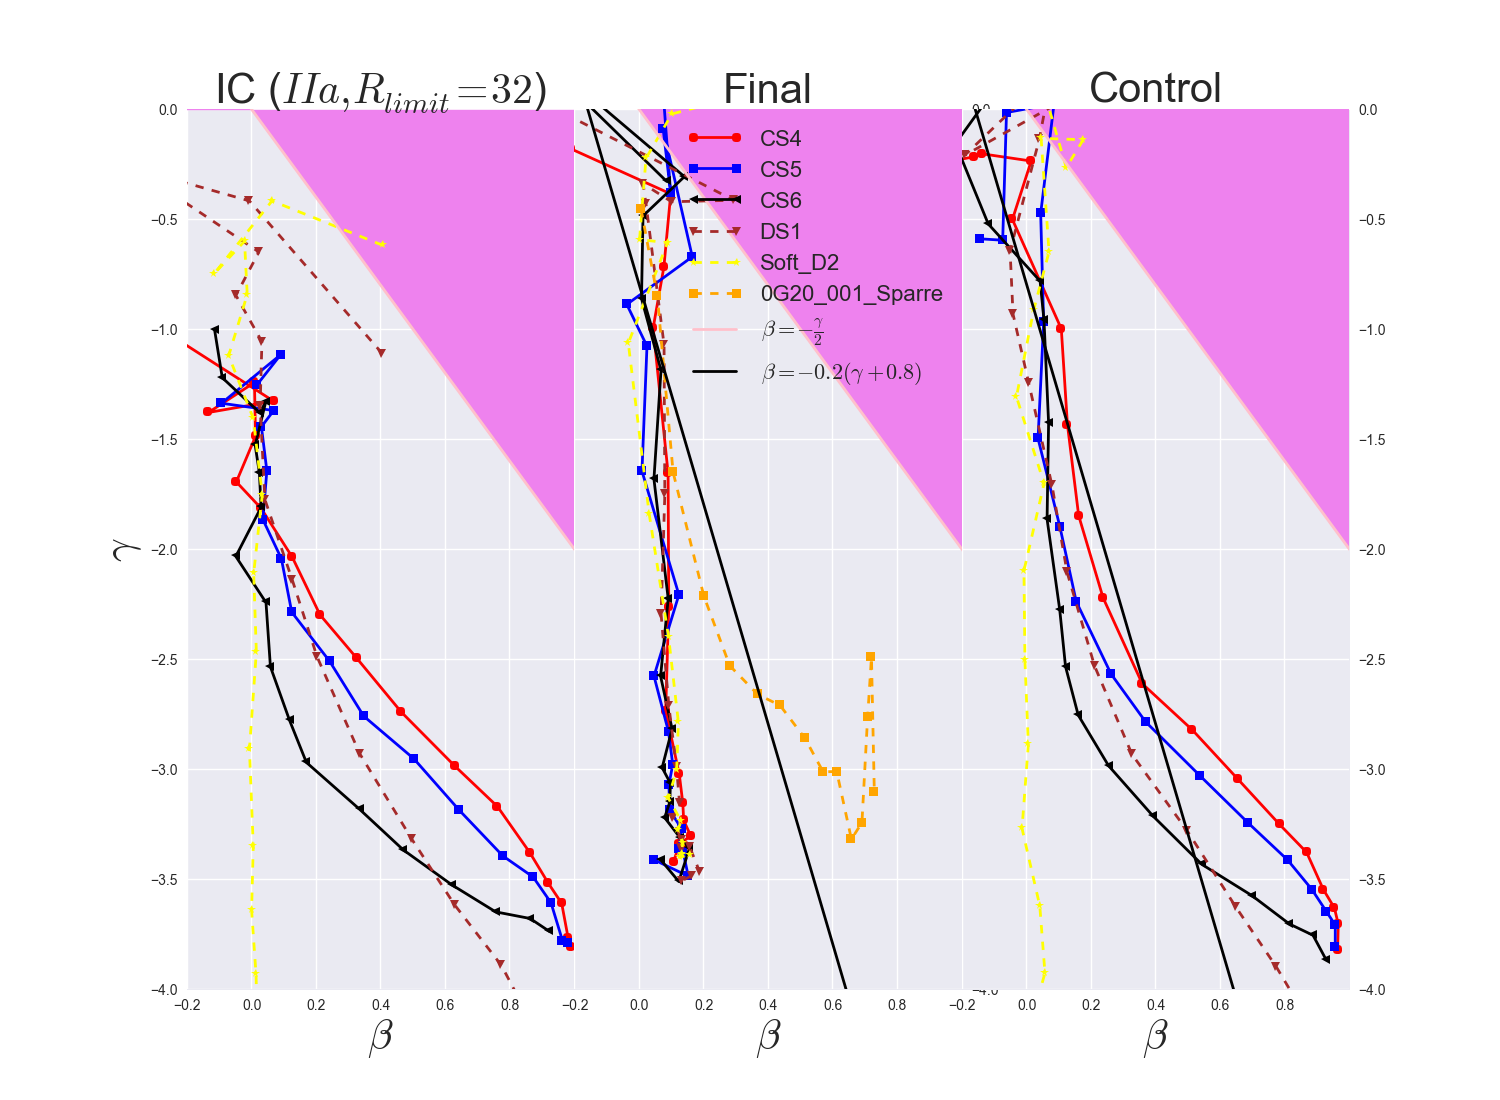
\includegraphics[width=1.0 cm]{img/beta_vs_gamma_CS4CS5CS6DS1D2_Rlimit32.png}
\caption{Attractor plot in the ($\beta$,$\gamma$)-space for Sim. IIa of stable structures $CS_4$, $CS_5$, $CS_6$, $DS_1$ and $D_2$. Structures are cut off at a radius of 32 times the scale radius. 20 radial bins are used. The left panel shows how the initial conditions spread out and fill up a large volume in the stable region of the Jeans parameter space spanned by $\beta$ and $\gamma$. This makes the attractor very apparent in the middle panel where structures are driven towards $\beta = 0.1$ in the outer regions. Final products are shown together with a final product from a sim. of type I performed by S.H. Hansen and M. Sparre for comparison. Also shown is the linear $\beta$-$\gamma$ relation discovered by Hansen and Moore (2006) for comparison. The pink upper right area is found to be an unstable region by An and Evans (2006).The control runs which are simulated with no perturbations interfering can be seen in the right panel. They show no significant departure from the initial conditions shown in the left panel.}
\label{fig:test}
\end{figure}

\begin{figure}[!htbp]
\centering
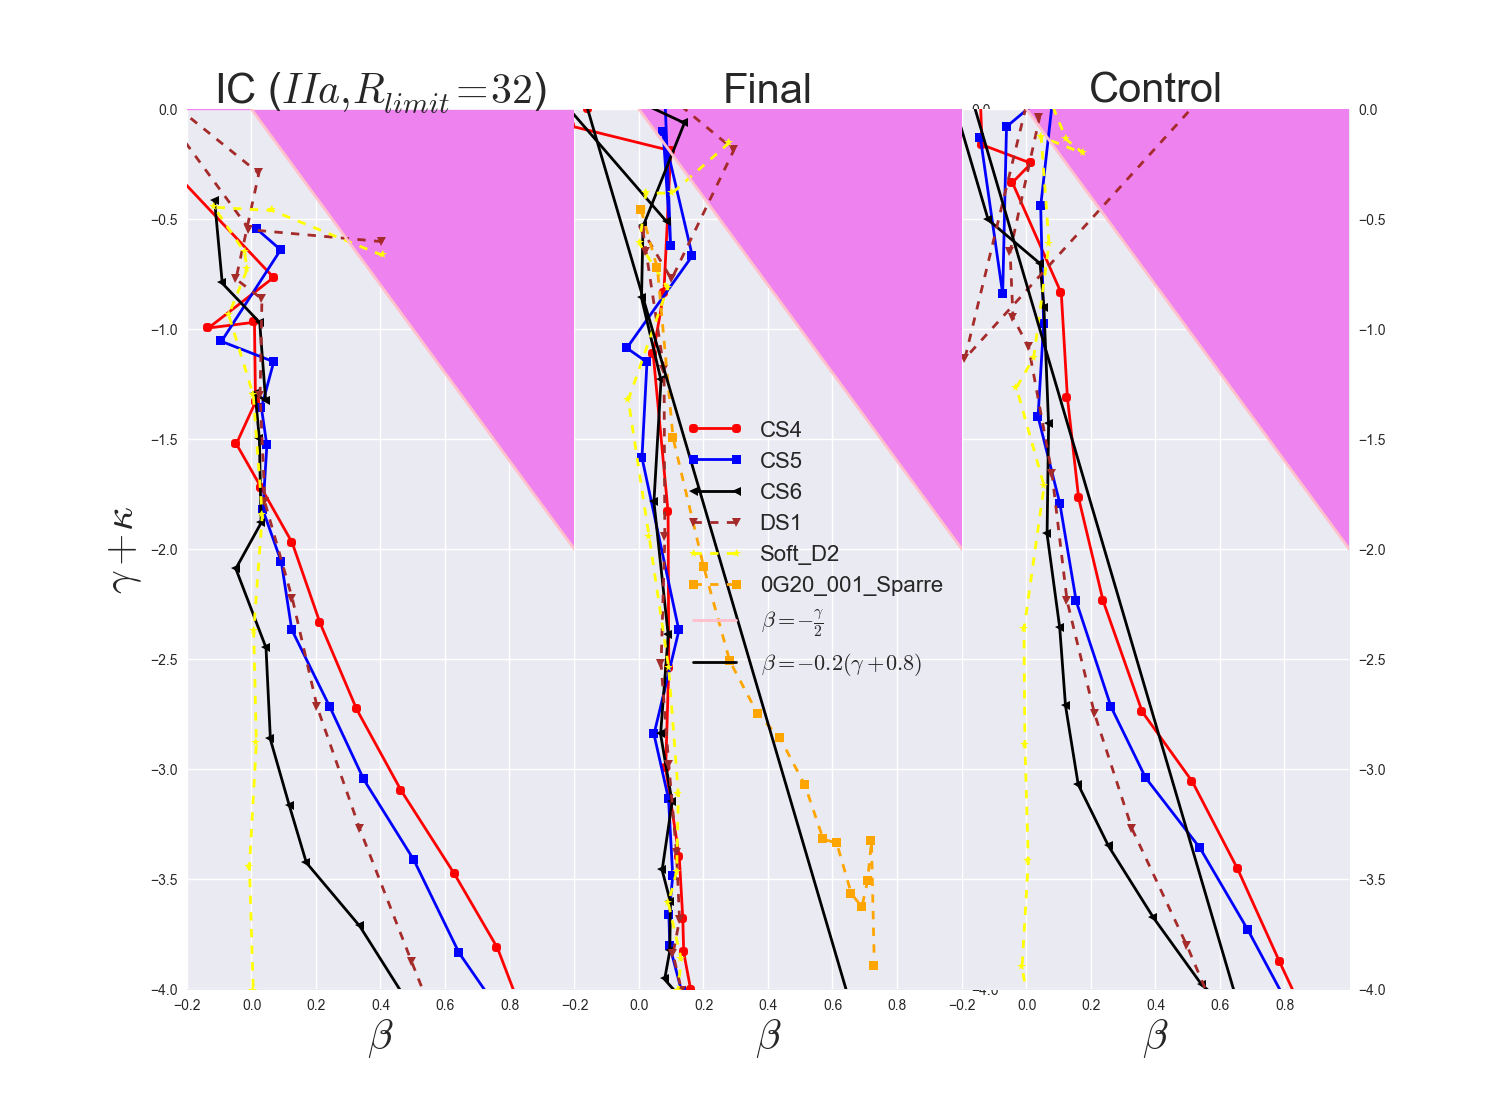
\includegraphics[width=1.0 cm]{img/beta_vs_gamma_plus_kappa_CS4CS5CS6DS1D2_Rlimit32.png}
\caption{Attractor plot in the ($\beta$,$\gamma + \kappa$)-space for Sim. IIa of stable structures $CS_4$, $CS_5$, $CS_6$, $DS_1$ and $D_2$.
Structures are cut off at a radius of 32 times the scale radius. 20 radial bins are used. In this projection the attractor is still clearly seen. We still compare it with the results found by others. The control runs which are simulated with no perturbations interfering can be seen in the right panel. They show no significant departure from the initial conditions shown in the left panel.}
\label{fig:test}
\end{figure}

\subsubsection{IIb: Energy exchange (radial velocity perturbations)}
\textbf{Using structures $CS_4$ and $D_2$, this simulation perturbs only the radial velocities of particles. Specifically, for all of these structures the total velocities inside spherical bins is perturbed for each of its particles by multiplying those given particles radial velocities ($v_r$) by random numbers in the range $[0.7, 1.3]$ (corresponding to perturbing the kinetic energies by random numbers in the range $\frac{1}{2}\cdot[0.49, 1.69]$), taken from the continuous uniform distribution. Following this exchange of kinetic energies between particles in fixed spherical bins, a normalization factor is applied to the total velocities, which ensures energy conservation. it has the same functional form as the one applied in sim. IIa, but will yield different numerical values as sim. $II_b$ does not perturb all three spherical velocities but only the radial one. The normalization factor will thus be smaller in this sim. After these velocity kicks the structures are simulated under their self gravity allowing them to flow a bit under their new velocities. This procedure is then repeated for a total of 20 runs (with one initial run where there is no perturbation. This allows the OM models to reach equilibrium, as they are not perfectly equilibrated when set up as OM models. It is done for Edd structures as well to be certain of equilibrium before any perturbations take effect). After the first 10 runs, the random number range is unchanged but the runs 11 $\rightarrow$ 20 are given longer timespans ($t_{sim} = 500$ corresponding to 5 dynamical times at $r = 12.7r_s$) to allow structures more flow.} \\ \\

Starting from the Cartesian quantities (coordinates and velocities) one of the first steps in the algorithm used for the perturbations is to perform a transformation into spherical quantities. This can be done by applying a function F which maps real values from the cartesian domain $R^3$ onto the spherical range $R^+ \times [0,\pi] \times [0,2\pi)$. F has the components: \\ 

\begin{align*}
R          & = \sqrt{x^2+y^2+z^2} \\
\theta     & = arccos(\frac{z}{R}) \\
\phi       & = arctan(\frac{y}{x}) \\
v_R        & = sin(\theta)cos(\phi)v_x+sin(\theta)sin(\phi)v_y+cos(\theta)v_z \\
v_{\theta} & = cos(\theta)cos(\phi)v_x+cos(\theta)sin(\phi)v_y-sin(\theta)v_z \\
v_{\phi}   & = - sin(\phi)v_x + cos(\phi)v_y \\
\end{align*}

The coordinate transformation from Cartesian to spherical curvilinear coordinates has the following Jacobian matrix:

\begingroup
\renewcommand*{\arraystretch}{2.5}
\begin{equation}
J_F(x,y,z) = 
\begin{bmatrix}
\dfrac{\partial R}{\partial x} & \dfrac{\partial R}{\partial y} & \dfrac{\partial R}{\partial z} \\ 
\dfrac{\partial \theta}{\partial x} & \dfrac{\partial \theta}{\partial y} & \dfrac{\partial \theta}{\partial z} \\ 
\dfrac{\partial \phi}{\partial x} & \dfrac{\partial \phi}{\partial y} & \dfrac{\partial \phi}{\partial z} 
\end{bmatrix} =
\begin{bmatrix}
\dfrac{x}{R} & \dfrac{y}{R} & \dfrac{z}{R} \\ 
0            &   0          & -\dfrac{1}{\sqrt{R^2-z^2}} \\ 
-\dfrac{y}{x^2+y^2} &  \dfrac{x}{x^2+y^2} & 0 
\end{bmatrix}
\end{equation}
\endgroup

The determinant of this Jacobian matrix is $\frac{1}{\sqrt{R^2-z^2}}$

Now the spherical velocities are ready to be manipulated inside the number bins.
Radial velocities are randomized as described above, and the speed is found as
$ v_{tot} = \sqrt{v_R^2 + R^2v_{\theta}^2 + R^2v_{\phi}^2sin(\theta)^2}$.
Some of the particles might become gravitationally unbound after this procedure. This is checked and any such unbound particles are rebound by multiplying their new randomized radial velocity component by another random number in the range [0.8,1.0] and then a normalization factor of $\sqrt[|\Phi|]{K_{rand}}$, where $|\Phi|$ is the numerical value of the gravitational potential inside any particular bin and $K_{rand}$ is the total kinetic energy of the unbound particles inside that bin.
A final normalization factor is then applied to all particles inside any given bin in order to obtain energy conservation. This factor is given by $K_{ratio} = \sqrt[<K_{init}>]{<K_{final}>}$, where $<K_{init}>$ is the initial total kinetic energy of the particles inside that bin and $<K_{final}>$ is the final total kinetic energy of the particles inside that bin. The operation to ensure energy conservation thus becomes: $ v_{R,final} = v_{R,init} \cdot K_{ratio} $, where $v_{R,init}$ are the velocities prior to the perturbation.  

Final step of the perturbation algorithm is to transform spherical quantities back to Cartesian (so that the perturbed structure can be saved as a snapshot-file of correct format which the GADGET-2 code can then read and simulate). This can be done by applying another function F, which maps the spherical domain $R^+ \times [0,\pi] \times [0,2\pi)$ onto the Cartesian range $R^3$. This new F giving the back-transformation has the components: \\ 

\begin{align*}
x   &= Rsin(\theta)cos(\phi) \\
y   &= Rsin(\phi)sin(\theta) \\
z   &= Rcos(\theta) \\
v_x &= sin(\theta)cos(\phi)v_R + cos(\phi)cos(\theta)v_{\theta} - sin(\phi)v_{\phi} \\
v_y &= sin(\phi)sin(\theta)v_R + sin(\phi)cos(\theta)v_{\theta} + cos(\phi)v_{\phi} \\
v_z &= cos(\theta)v_R - sin(\theta)v_{\theta}
\end{align*}

The coordinate transformation from spherical to Cartesian coordinates has the following Jacobian matrix:

\begingroup
\renewcommand*{\arraystretch}{2.5}
\begin{equation}
J_F(r,\theta,\phi) = 
\begin{bmatrix}
\dfrac{\partial x}{\partial R} & \dfrac{\partial x}{\partial \theta} & \dfrac{\partial x}{\partial \phi} \\ 
\dfrac{\partial y}{\partial R} & \dfrac{\partial y}{\partial \theta} & \dfrac{\partial y}{\partial \phi} \\ 
\dfrac{\partial z}{\partial R} & \dfrac{\partial z}{\partial \theta} & \dfrac{\partial z}{\partial \phi} 
\end{bmatrix} =
\begin{bmatrix}
sin(\theta)cos(\phi) &  Rcos(\theta)cos(\phi)  & -Rsin(\theta)sin(\phi)  \\ 
sin(\theta)sin(\phi) &  Rcos(\theta)sin(\phi)  &  Rsin(\theta)cos(\phi)  \\ 
cos(\theta)          & -Rsin(\theta)  &  0 
\end{bmatrix}
\end{equation}
\endgroup

The determinant of this Jacobian matrix is $R^2sin(\theta)$.

\begin{figure}[!htbp]
\centering
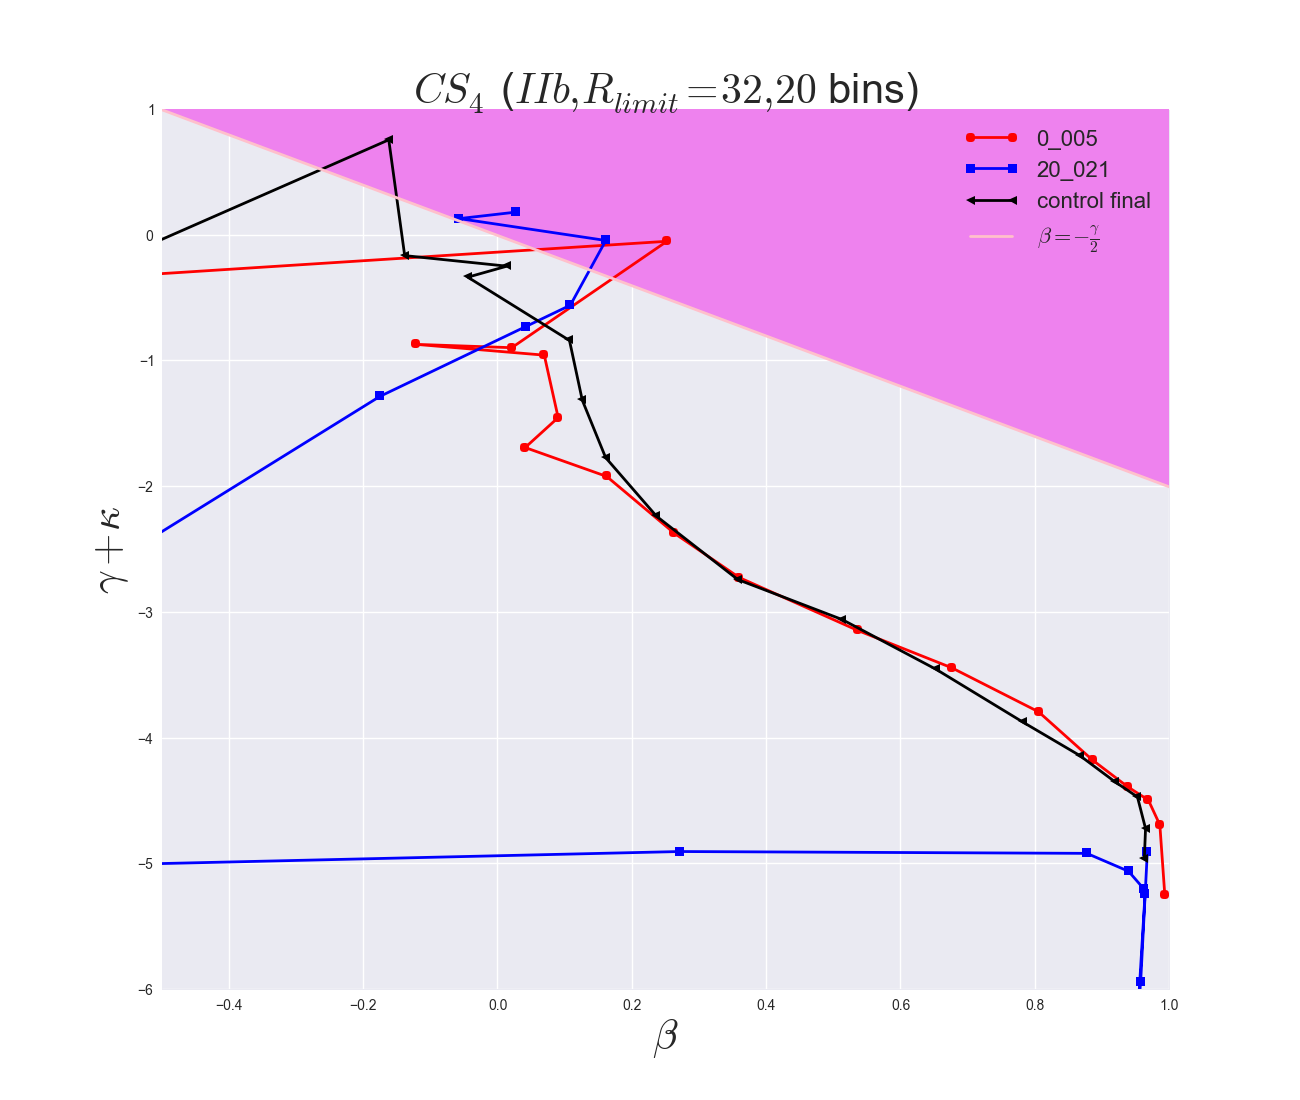
\includegraphics[width=1.0\linewidth]{img/beta_vs_gamma_plus_kappa_IIb_CS4_Rlimit32.png}
\caption{$\gamma + \kappa$ vs. $\beta$ for IC, final product and control run of sim. IIb, of stable structure $CS_4$.
Structures are cut off at a radius of 32 times the scale radius. 20 radial bins are used.
No attractor is found. This agrees with work done by others [4]. The conclusion here must be then that not all perturbations will work when trying to reveal natures attractors. In [4] this is compared to a ball being continuously kicked uphill. The ball might wish to fall down (flow) but never get a chance to if it is repeatedly being kicked upwards (e.g. radially perturbed as in this case). Perhaps this experiment is just not in agreement with any physical process.}
\label{fig:test}
\end{figure}

\begin{figure}[!htbp]
\centering
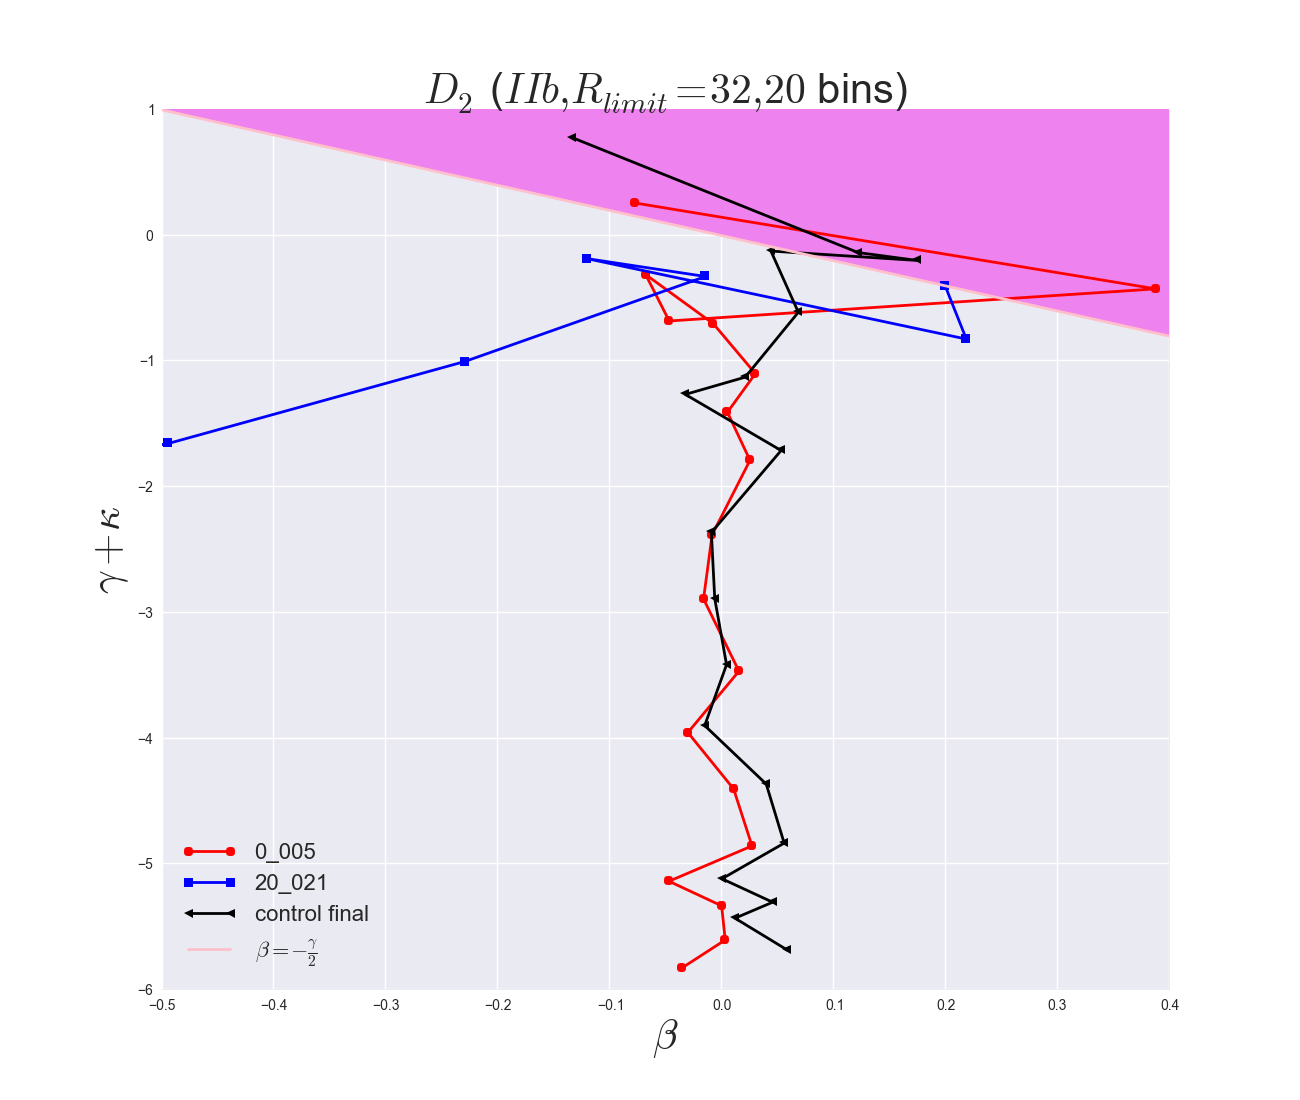
\includegraphics[width=1.0\linewidth]{img/beta_vs_gamma_plus_kappa_IIb_D2_Rlimit32.png}
\caption{$\gamma + \kappa$ vs. $\beta$ for IC and final product of sim. $II_b$ of structure $D_2$.
Structures are cut off at a radius of 32 times the scale radius. 20 radial bins are used.
No attractor is found. This agrees with work done by others [4]. The conclusion here must be then that not all perturbations will work when trying to reveal natures attractors. In [4] this is compared to a ball being continuously kicked uphill. The ball might wish to fall down (flow) but never get a chance to if it is repeatedly being kicked upwards (e.g. radially perturbed as in this case). Perhaps this experiment is just not in agreement with any physical process.}
\label{fig:test}
\end{figure}

\subsubsection{IIc: Energy exchange (tangential velocity perturbations)}
\textbf{Using structures $CS_4$ and $D_2$, this simulation perturbs only the tangential velocities of particles. Specifically, for all of these structures the total velocity inside spherical bins is perturbed for each of its particles by multiplying those given particles tangential velocities $v_{\theta}$ and $v_{\phi}$ by random numbers in the range $[0.9, 1.1]$ before each of the first ten simulations (each lasting for a duration of 1 $t_{dyn}$ at $r = 12.7 r_s$) and 
random numbers in the range $[0.7, 1.3]$ before each of the next twenty (for $D_2$) or ten (for $CS_4$) simulations (each of which this time lasting for a duration of 5 $t_{dyn}$ at $r = 12.7 r_s$, allowing structures more flow) (corresponding to perturbing the kinetic energies by random numbers in the range $\frac{1}{2}\cdot[0.49, 1.69]$), taken from the continuous uniform distribution. Following this exchange of kinetic energies between particles in fixed spherical bins, a normalization factor is applied to the total velocities, which ensures energy conservation. it has the same functional form as the one applied in sim. $II_a$, but will yield different numerical values as sim. IIc does not perturb all three spherical velocities but only the two tangential ones. The normalization factor will thus be smaller in IIc than the one utilized in IIa but on average larger than the one in $II_b$. After these velocity kicks the structures are simulated under their self gravity allowing them to flow a bit under their new velocities. This procedure is then repeated for a total of 20 runs for $CS_4$ and 30 runs for $D_2$ (with one initial run where there is no perturbation. This allows the OM models to reach equilibrium, as they are not perfectly equilibrated when set up as OM models. It is done for Edd structures as well to be certain of equilibrium before any perturbations take effect). $CS_4$ only gets 20 runs as it does not change significantly and thus already seem to start out at a stable point. $D_2$ is however simulated for 30 runs at it changes significantly after each simulation. After 20 runs it has reached a stable point where the next 10 runs until run 30 has no real effect on $D_2$ at all.} \\ \\

Similarly to $II_b$, the $II_c$ sim. transforms Cartesian into spherical quantities, divides the structure into particle number bins, perturbs and normalize velocities and energy, and finally transforms back to Cartesian form followed by saving into a new snapshotfile which can then be read and simulated by the GADGET-2 code.

\begin{figure}[!htbp]
\centering
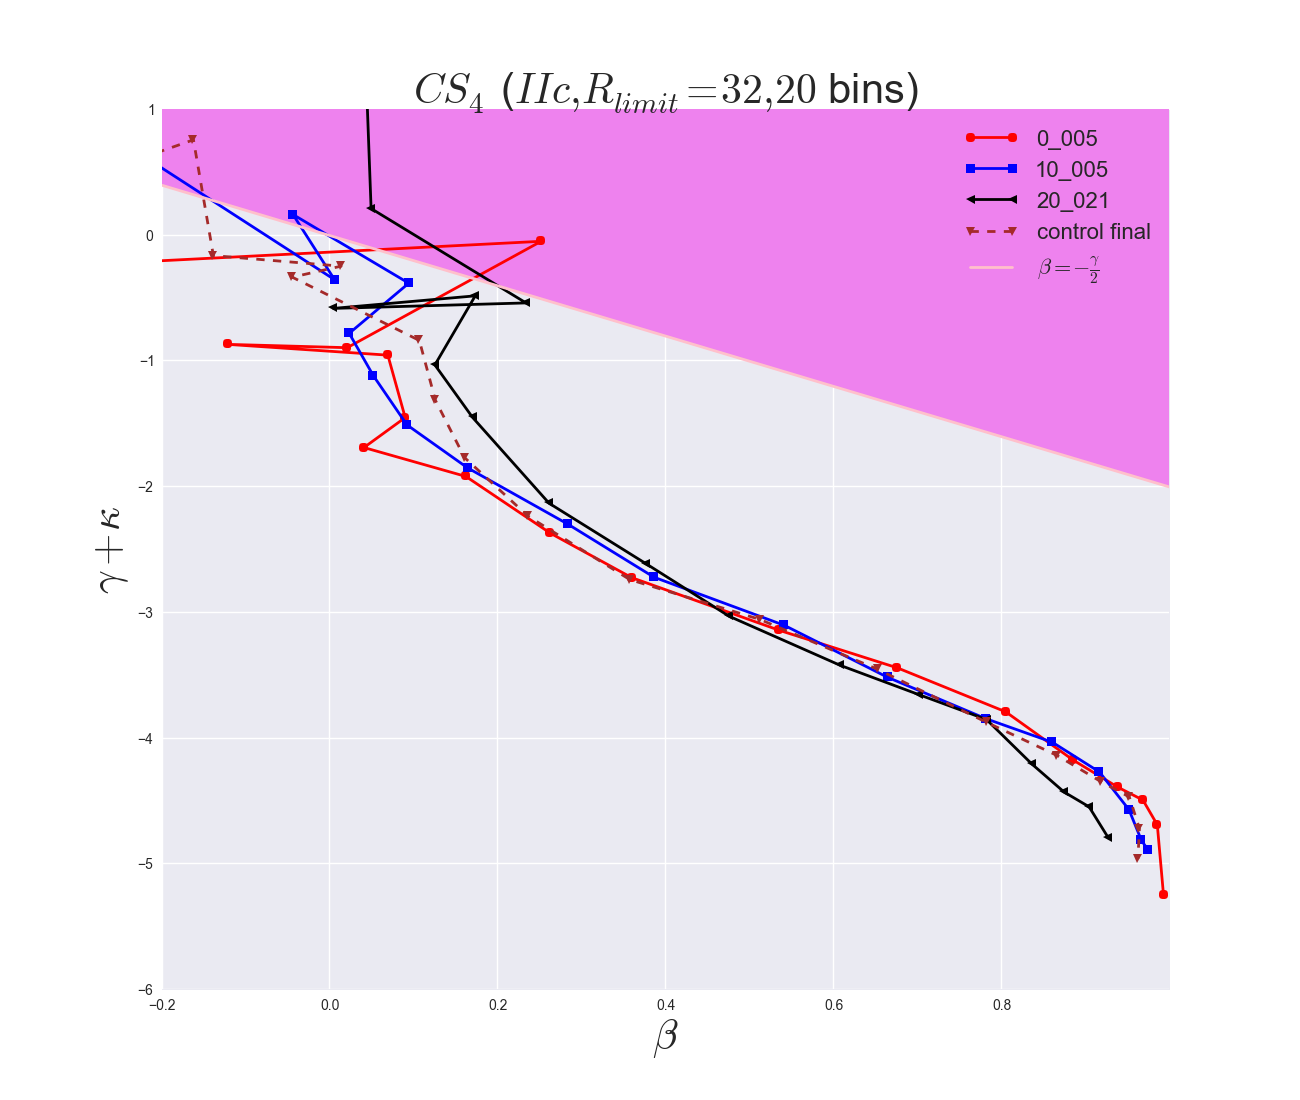
\includegraphics[width=1.0\linewidth]{img/beta_vs_gamma_plus_kappa_IIc_CS4_Rlimit32.png}
\caption{$\gamma + \kappa$ vs. $\beta$ for IC, 10, final product and control run of sim. IIc of structure $CS_4$. Structures are cut off at a radius of 32 times the scale radius. 20 radial bins are used.
No change is seen at any part of this structure from $\beta = 0.2$ and upwards. The inner fluctuations where $\beta$ is smaller can be attributed to numerical noise as the radii here moves close to the softening length of the sim. The lack of change is most probably that structure $CS_4$ already starts out very close to the attractor and therefore remains here. When analyzing the shape of this structure up close it is seen to fulfill the attractor values already found in [4], namely $(\gamma + \kappa) = -8\beta$ for smaller radii and $(\gamma + \kappa) = -0.7-4\beta$ for larger radii.}
\label{fig:test}
\end{figure}

\begin{figure}[!htbp]
\centering
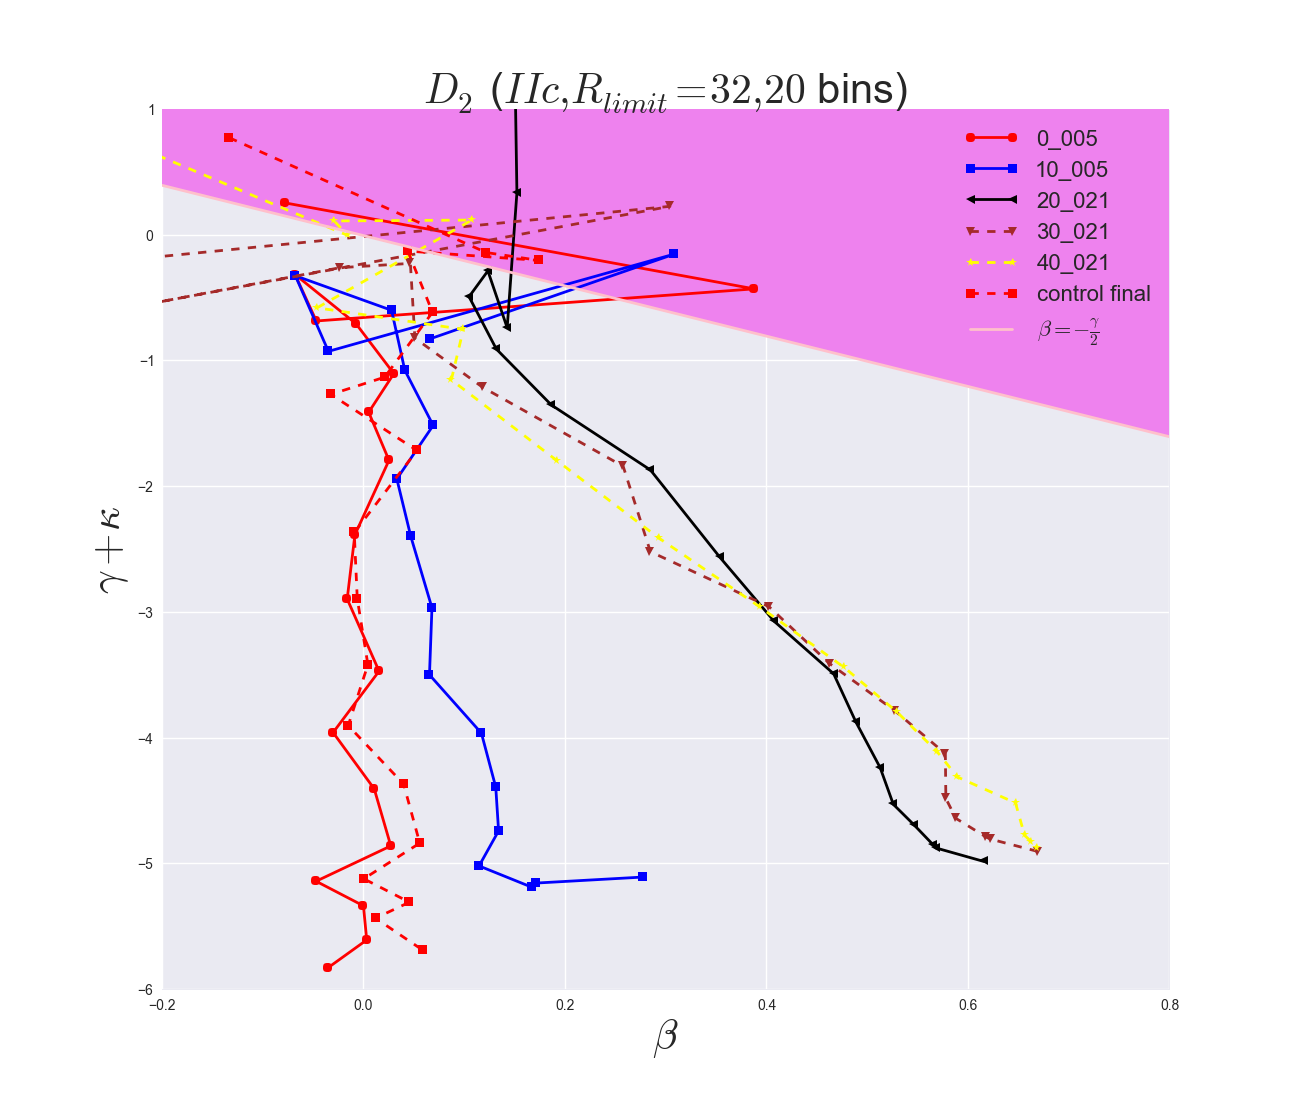
\includegraphics[width=1.0\linewidth]{img/beta_vs_gamma_plus_kappa_IIc_D2_Rlimit32.png}
\caption{$\gamma + \kappa$ vs. $\beta$ for IC, 10, 20, 30, final product and control run of sim. IIc of structure $D_2$. Structures are cut off at a radius of 32 times the scale radius. 20 radial bins are used.
The IC is seen to start out as isotropic ($D_2$ is generated by Eddingtons inversion method) but then systematically exhibits flow toward the same attractor as seen present in the previous figure for the $CS_4$ structure. This structure is given more simulation time than $CS_4$ in order to follow its evolution more fully. It is indeed seen to move closer and closer to the characteristic s-shaped attractor curve found by others [4]. It is therefore safe to conclude that sim. IIc (perturbing tangential velocities) will drive structures towards the attractor previously found.}
\label{fig:test}
\end{figure}

\subsubsection{IId: Energy exchange (speed perturbations)}
\textbf{Using structures $CS_4$ and $D_2$, this simulation perturbs only the speed of particles and not the direction of the velocity vector. Specifically, for all of these structures the total velocities inside spherical bins is perturbed for each of its particles by multiplying those given particles cartesian velocities ($v_x$, $v_y$ and $v_z$) by the same random numbers for each three directions (thus only changing the speed) in the range $[0.7, 1.3]$ (corresponding to perturbing the kinetic energies by random numbers in the range $\frac{1}{2}\cdot[0.49, 1.69]$), taken from the continuous uniform distribution. Following this exchange of kinetic energies between particles in fixed spherical bins, a normalization factor is applied to the total velocities, which ensures energy conservation. it has the same functional form as the one applied in sim. IIa. After these velocity kicks the structures are simulated under their self gravity allowing them to flow a bit under their new velocities. This procedure is then repeated for a total of 20 runs (with one initial run where there is no perturbation. This allows the OM models to reach equilibrium, as they are not perfectly equilibrated when set up as OM models. It is done for Edd structures as well to be certain of equilibrium before any perturbations take effect). After the first 10 runs, the random number range is unchanged but the runs 11 $\rightarrow$ 20 are given longer timespans ($t_{sim} = 500$ corresponding to 5 dynamical times at $r = 12.7r_s$) to allow structures more flow.} \\ \\

\begin{figure}[!htbp]
\centering
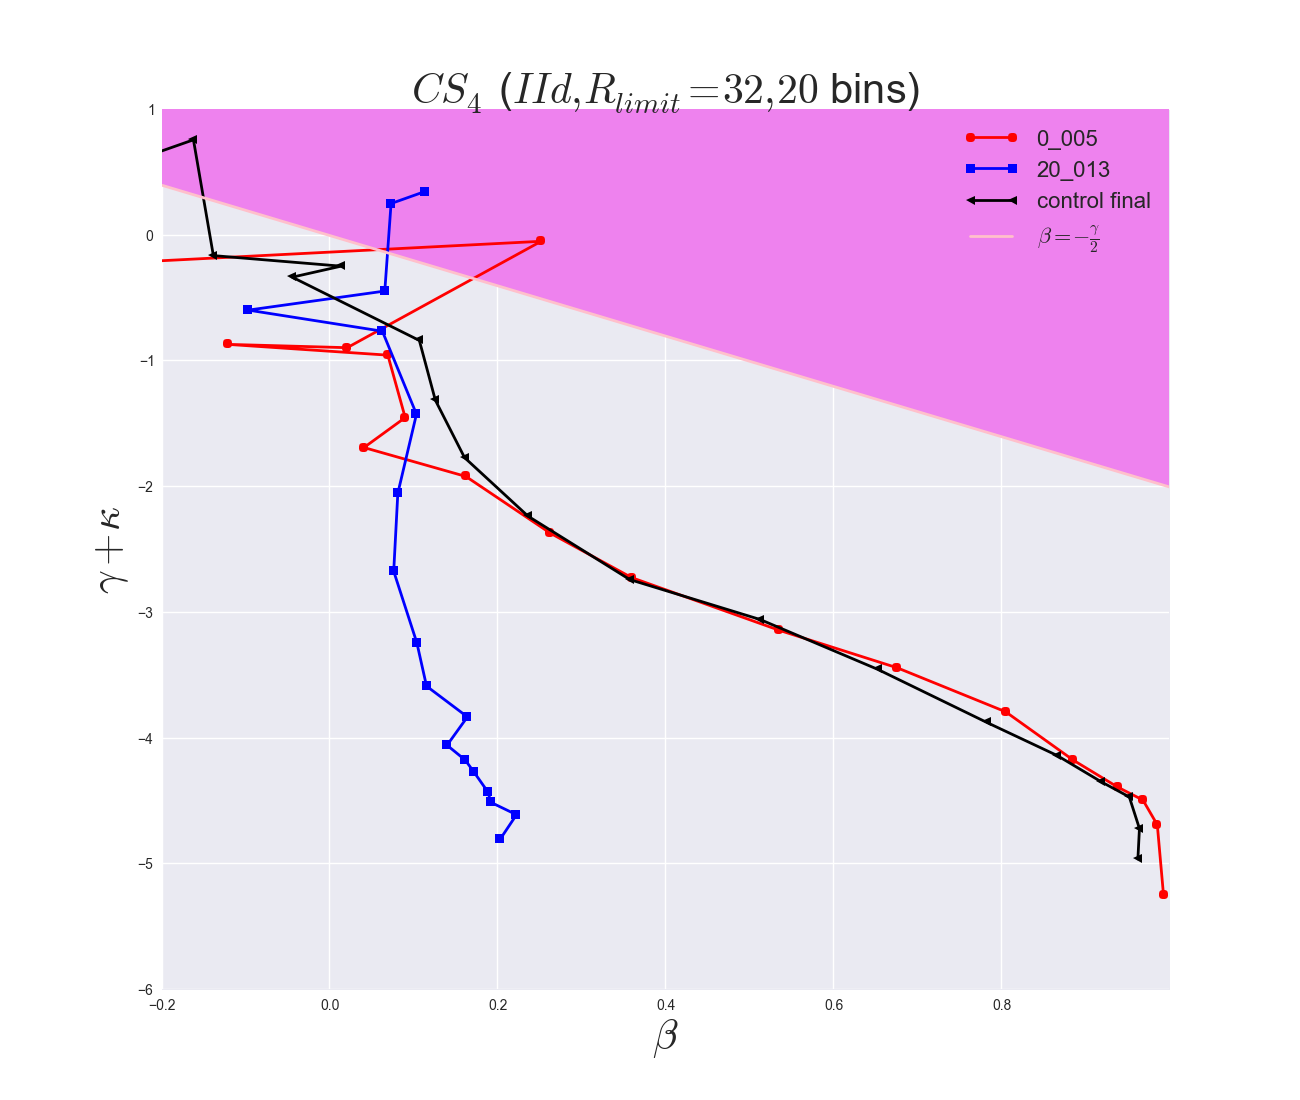
\includegraphics[width=1.0\linewidth]{img/beta_vs_gamma_plus_kappa_IId_CS4_Rlimit32.png}
\caption{$\gamma + \kappa$ vs. $\beta$ for IC and final product of sim. $II_d$ of structure $CS_4$.
Structures are cut off at a radius of 32 times the scale radius. 20 radial bins are used.
The attractor is present and can be seen for the final structure 20$\_$013 which has been driven towards $\beta = 0.1$ in the outer regions. The pink upper right area is found to be an unstable region by An and Evans (2006).The control runs which are simulated with no perturbations interfering can be seen as well. They show no significant departure from the initial conditions.}
\label{fig:test}
\end{figure}

\begin{figure}[!htbp]
\centering
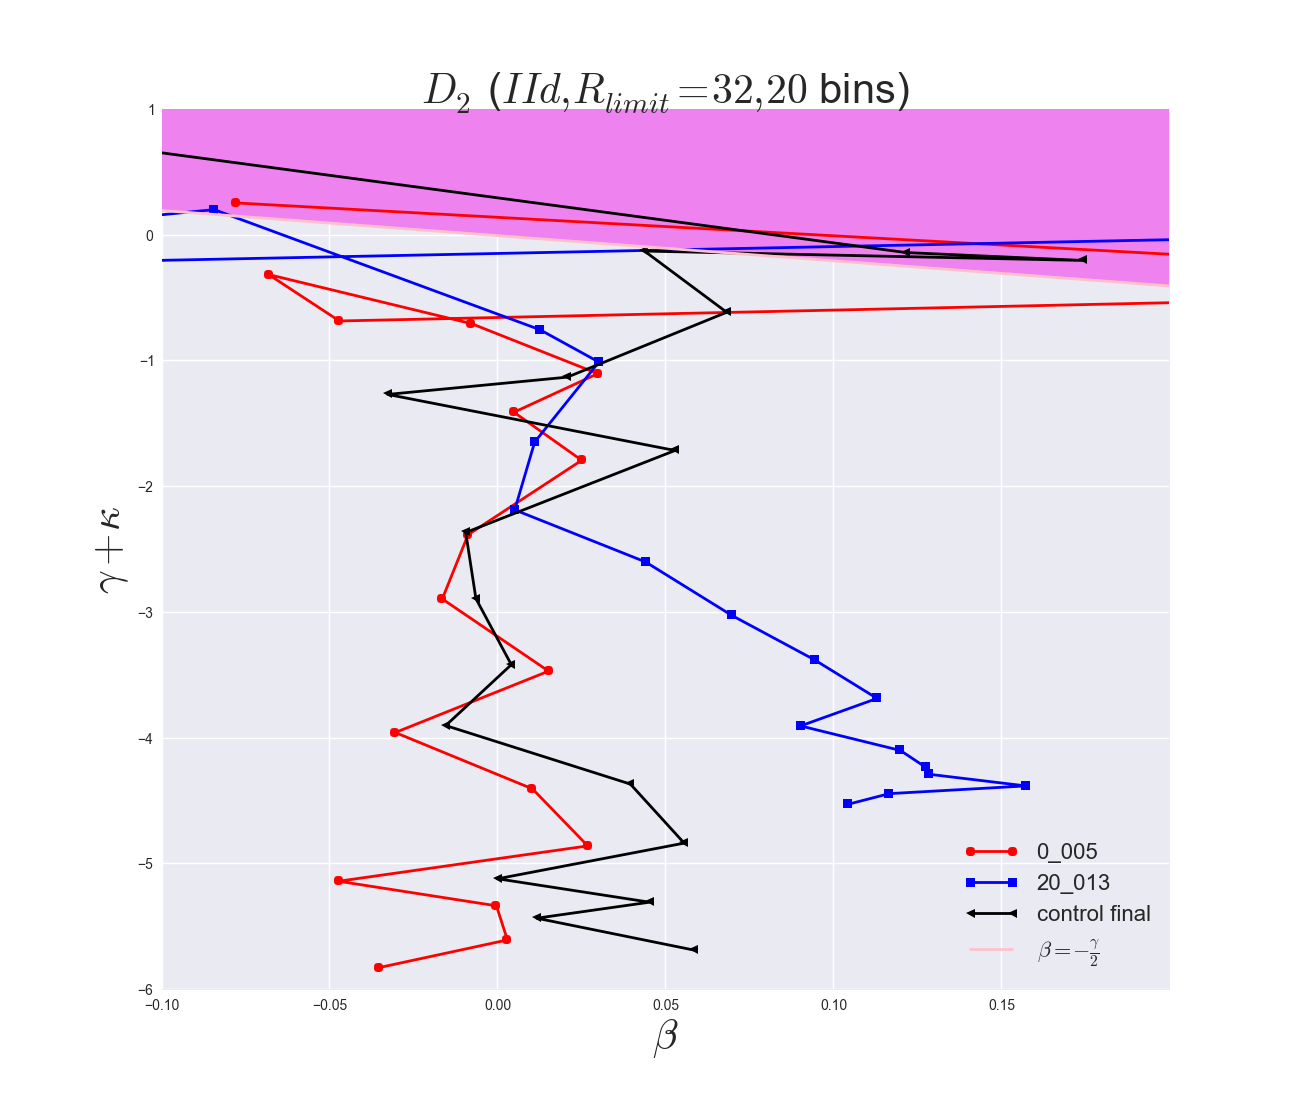
\includegraphics[width=1.0\linewidth]{img/beta_vs_gamma_plus_kappa_IId_D2_Rlimit32.png}
\caption{$\gamma + \kappa$ vs. $\beta$ for IC and final product of sim. $II_d$ of structure $D_2$.
Structures are cut off at a radius of 32 times the scale radius. 20 radial bins are used.
The attractor is present and can be seen for the final structure 20$\_$013 which has been driven towards $\beta = 0.1$ in the outer regions. The pink upper right area is found to be an unstable region by An and Evans (2006).The control runs which are simulated with no perturbations interfering can be seen as well. They show no significant departure from the initial conditions.}
\label{fig:test}
\end{figure}

\textbf{We have so far seen the ICs plugged into sim. I and II and the outcome of this procedure.
The next section highlights a few features from these sims. such as a particles trajectory when tracking it through subsequent snapshots during a simulation, effects found when zooming in on different radial domains, how softening length introduces numerical noise in the inner region leading us to make a inner cut and how outer parts of structures have insufficient time to reach equilibrium due to the large inter-particle distances leading us to make an outer cut. We thus obtain a valid range of trust where all structures can be safely analyzed. The next section concludes with a mention of OM models and their inability to reach any attractor, in good agreement with previous work done by others.}